\section{A far wake instability for intermediate $\AR$s}

For the circular cylinder case it is well known \citep{vorobieff-goergiev-ingber-2002,kumar-mittal-2012} that the primary vortex street in the near wake transitions into a two-layered vortex street in the intermediate wake, followed by a transition from the two-layered vortices to a secondary vortex steet in the far wake.

The physical mechanism for the first transition was investigated by \cite{durgin-karlsson-1971}, \cite{karasudani-funakoshi-1994} and \cite{dynnikova-guverntuk-2016}. According to their results the breakdown of the primary vortex street is the result of the convection of vorticity within a vortex by the other vortices of the street. The physical mechanism for the second transtion has been attributed to the hydrodynamic instability of the mean wake flow \citep{cimbala-nagib-roshko-1988,williamson-prasad-1993}, and to the convective instability of the mean wake flow \citep{kumar-mittal-2012}.

The streamwise location for the second transition has been largely examined over the last years. For example \cite{inoue-yamazaki-1999} and  \cite{vorobieff-etal-2002} by means of two-dimensional numerical simulations and soap-film experiments increased the Reynolds number uo to $Re=1000$. They observed that the streamwise location of the second transition moved upstream with increasing $Re$, with a proposed law for the transition location of $\sim Re^{-1/2}$. 

More recently, \cite{jiang-cheng-2019} provided a detailed investigation of the far wake instabilities of the flow past a circular cylinder using two-dimensional simulations. They observed that the transition to the secondary vortex street is driven by two different processes depending on the Reynolds number. For small $R$, the transition process is dictated by the merging of two same-sign vortices, while at larger $Re$ it is driven by the pairing of two opposite-sign vortices followed by the merging of the paired vortices.


\cite{thompson-etal-2014} consdiered the flow past two-dimensional elliptic cylinders with the major axis placed normal to the flow direction, ranginf from a circular cylinder to a flat plate placed perpendicular to the incoming flow. They investigated the developement of the secondary vortex street for different geometries. At $Re=100$, tor the cyrcular cylinder they observed that the near wake is the classical K\'{a}rm\'{a}n vortex street, that further downstream develops into a two-layered wake. Moving downstream, they observed that the clockwise and anticlockwise vortices diffuse and crossannihilate, leaving a featureless wake. Increasing $Re$ the same scenario is observed, with the two-layered wake arising more downstream. When decreasing $\AR$, instead, the observed that the transition process is accelerated. For example, for $\AR=0.5$ at $Re=200$ they observed that the transition from the K\'{a}rm\'{a} street to the two-layered street occurs within two diameters past the cylinder and that the stationary wake does not form at all. \textcolor{red}{Interestingly, they observed that for small $\AR$ as $Re$ increases the transition migrates upstreams and the developement of the mode A instability is suppressed. This shows that at smaller Reynolds number the near-wake is threedimensional. But then, increasing $Re$ the transition of the two-dimensional wake moves upstream and suppressed the global instability. A simila scenario with modes that become unstable and then stabilise again as $Re$ increases has been observed for the flow past rotating cyilinder \citep{rao-etal-2013,radi-etal-2013}. XX This is similar to what we do observe for $\AR=2.5$ apparently. Look at the base flow to further understand what happens. XX}


\cite{durgin-karlsson-1971} considered a von K\'{a}rma\'{a}n vortex street subjected to a deceleration. This modifies the ratio of longitudinal to lateral spacing between the vortices. They observed that the distortion of the individual vortices resultes in annihilation of concentrated vortex regions and creation of a stationary wake flow. This resulting wake flow is itself dynamically unstable and develops into a new vortex street of a different frequency form the initial one. They explained the breakdown of the initial vortex street with the convection of a concentrated vortex region due to the motion imposed by all the other vortices. In 1959 Taneda discovered that far downstream the original vortex street disappears and a new one of larger scales appears. His results were later confirmed by the observation of \cite{zdravkovich-1968} who photographed the vortex trails of three cylinders in close proximity. They considered this problem experimentaly, by looking at the vortex street generated from a cyrcular cylinder ad develerated by the presence of a downstream larger circular cylinder placed perpendicular to the first one and to the flow. Between the two cylinder they observed that the K\'{a}rm\'{a}n vortex street changes structure. More specifically, near the outside of the wake the measure a single frequency sinusouidal wake. \textcolor{red}{When the probe was moved closer to the centreline, they observed that a dominat second harmonic component arises. This is well documented i Kovasznay (1949) and Roshko (1953)}. When moving downstream they observed that the fluctuations become smaller and finally become not detectable. This corresponds to the two-layer region and is referred to as the calm region. Here no velocity fluctuations are visible in the centreline. The end of this calm region is detected by the development of a grwoing instability and the formation of a new vortex street with much larger widft and wavelength than the original. \textcolor{red}{They observed that the frequency of the primary and secondary wake exhibit a linear relation, see their figure 3}. A good way to recognise the primary vortex street, the calm region and the secondary vortex street is to look at the mean velocity at the centreline. Here $U$ exhibits a clear drop in the calm region, before recovering in the secondary vortex street. \textcolor{red}{What if we simply look at instantaneous snapshots? The problem is that the regions where the two vortex street are generated may change in time, so we do not have in this way a statistical information of the ``average'' points}. They measure the longitudinal shape of the vortex filaments by using correlations. In particular they detected the position of the vortex positions by looking at the zero correlation points. They observed that the vlaues of the downstream spacing $a$ between two shed vortices decreases by approximately $60\%$ along tha primary vortex street. \textcolor{blue}{How do we measure this? We can simply look at the local maxima of the vorticity for example. However, some references for example Hooker (1936) mentioned that this points is not exacly the same as the point where the fluid appears to rotate because of the vorticity diffusion}. This considerably devates form that of a vortex street in uniform flow which exhibits a realstively constant value in downstream spacing \citep{schaefer-eskinazi-1959}. They propose a model using a Hamel--Oseen vortex model for the vortices and observed that the arise of the calm region is related to the moment where $h/a<0.366$. In this case the part of the vortex outside the vortex street leads the inside part in the downstream direction. Therefore, these vortices starts deforming due to their mutual interaction and then, after deformed, they annihilate each other giving rise to the so-called calm region. They report that the calm regions consists (on average) of two adjactent layers of vorticity of opposite sigs. Here the mean velocity profiles are reminescent of the laminar wake formed behind a flat plate in a uniform stream. These shear layers are then unstable and give rise to the secondary vortex street. The scenario described by \cite{durgin-karlsson-1971} was later confirmed by the experimental work of \cite{karasudani-funakoshi-1994}.

\cite{taneda-1959} suggested that the origin of the secondary vortex street of large scale may be explained by the linear stability theory for the locoal mean wake profile, which changes slowly in the streamwise direction. Matsui and Okude (1982) and Okude and Matsui (1990) proposed that the secondary vortex street is formed by the pairing of the vortices in the primary vortex steet. That is, they claimed that the wavelength of the vortex street becomes larger as a result of the pairing of vortex regions, withoug actually going through a parallel shear flow state. However, successive results presented for example by \cite{karasudani-funakoshi-1994}. Indeed, by looking at the wavelengths of the primary and secondary vortex streets, i.e. $a_1$ and $a_2$ they do not observe that the ratio $a_2/a_1$ is close to $2$ for a wide range of $Re$, as expected in the case of vortex pairing. Similarly, the ratio of the frequencies $f_1/f_2$ is observed for decrease with increasing $Re$, again in contraddiction with the vortex pairing scenario where instead $f_1/f_2$ should be close to 2. 

\textcolor{red}{XX PLOT A ZOOM OF THE DIFFERENT FLOW REGIONS, TO SHOW THAT THE PRIMARY VORTEX STREET EVOLVES INTO A NEARLY PARALLEL SHEAR FLOW, BEFORE THE SECONDARY VORTEX STREET ARISES xx}

\textcolor{blue}{XX Can we detect the centre of the vortices to measure $h$ and $a$ using the local maxima of the vorticity?  I have to compute $h_1$ and $h_2$, i.e. the transverse spacing of neighbouring vortex regions of opposite signs in the primary and secondary wakes and $a_1$ and $a_2$, i.e. the longitudinal spacing of vortex regions of the same sign in the parimary and secondary vortex streets respectively XX} 

\cite{karasudani-funakoshi-1994} observed that since a nearly parallel flow is observed before the secondary vortex street, it is reasonable to predict that the formation of this vortex street is the result of the instability of the parallel flow, similarly to what predicted by \cite{taneda-1959} and \cite{cimbala-1988}. They used the data of \cite{fujimura-etal-1988} that calculated the linear stability of the parallel flow, approximating the velocity profiles with Gaussian cruves.

\cite{jhonson-thompson-hourigan-2004}

\cite{alksyuk-shkadova-shkadov-2012}

Apart from viscous diffusion, the geometric arrangement of the vortices in the vortex street determines whether is it predominately stable or whether it breaks fown into a parallel shear flow. \cite{durgin-karlsson-1971} defined a critical value of $h/a = 0.365$ where $h$ is the cross-wake spacing between positive and negative wake vortices, while $a$ is the separation between vortices of the same sign. Above this critical value, the vortices stretch our and aling with the downstreamw direction leading to a parallel shear flow. In turn, this mean shear flow can become unstable forming a secondary vortex street. This process was further investigated by \cite{karasudani-funakoshi-1994}.

Although the scope of the present work is not on this we report some results.

\begin{figure}
  %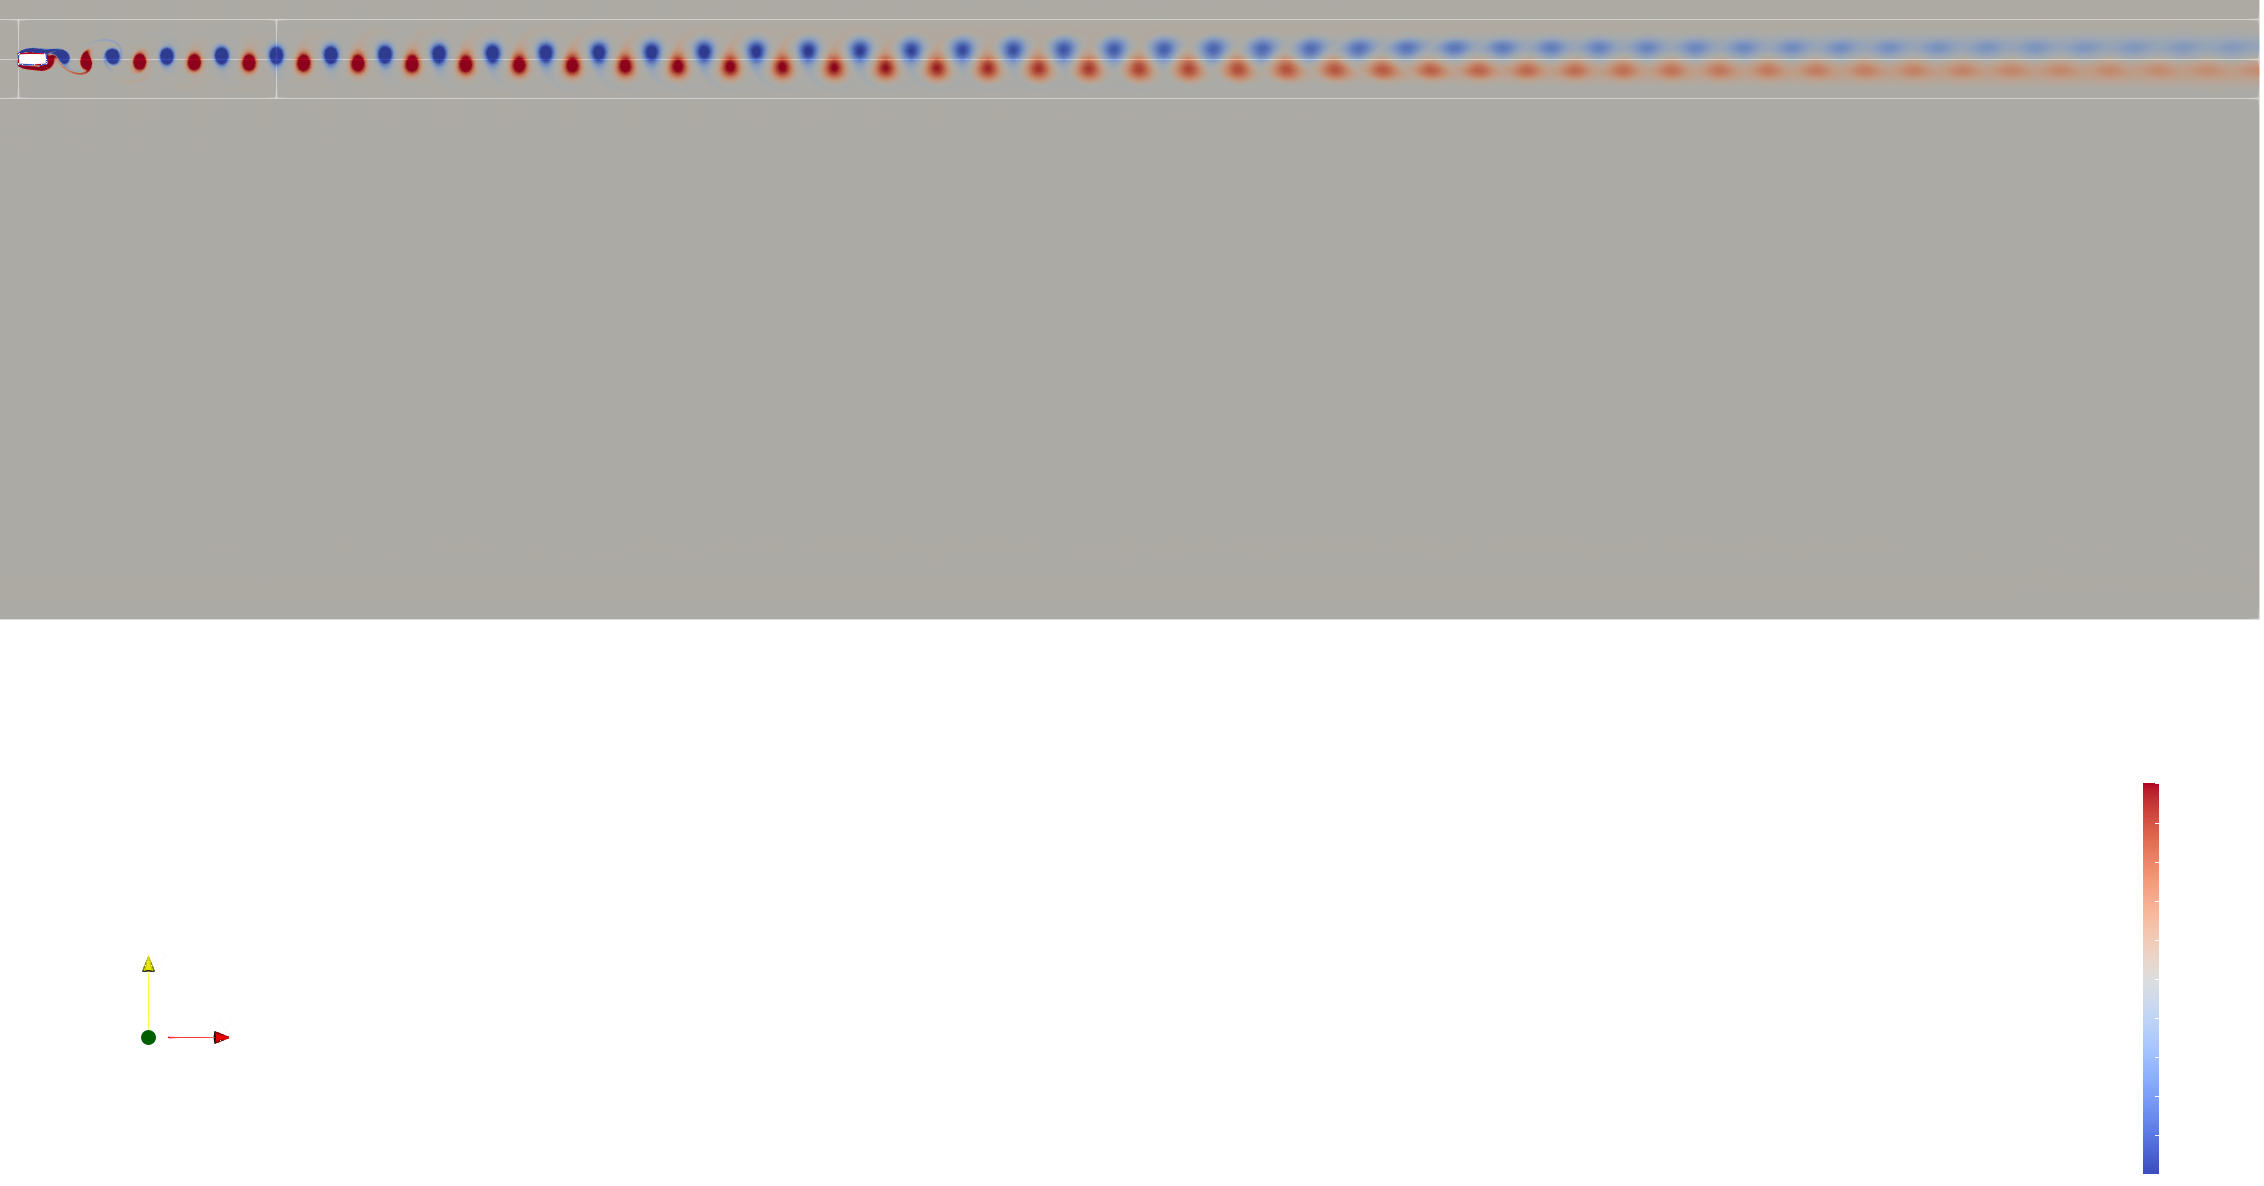
\includegraphics[trim={0 1060 0 0},clip,width=\textwidth]{./fig/appendix/AR2p5_Re450.png}
  %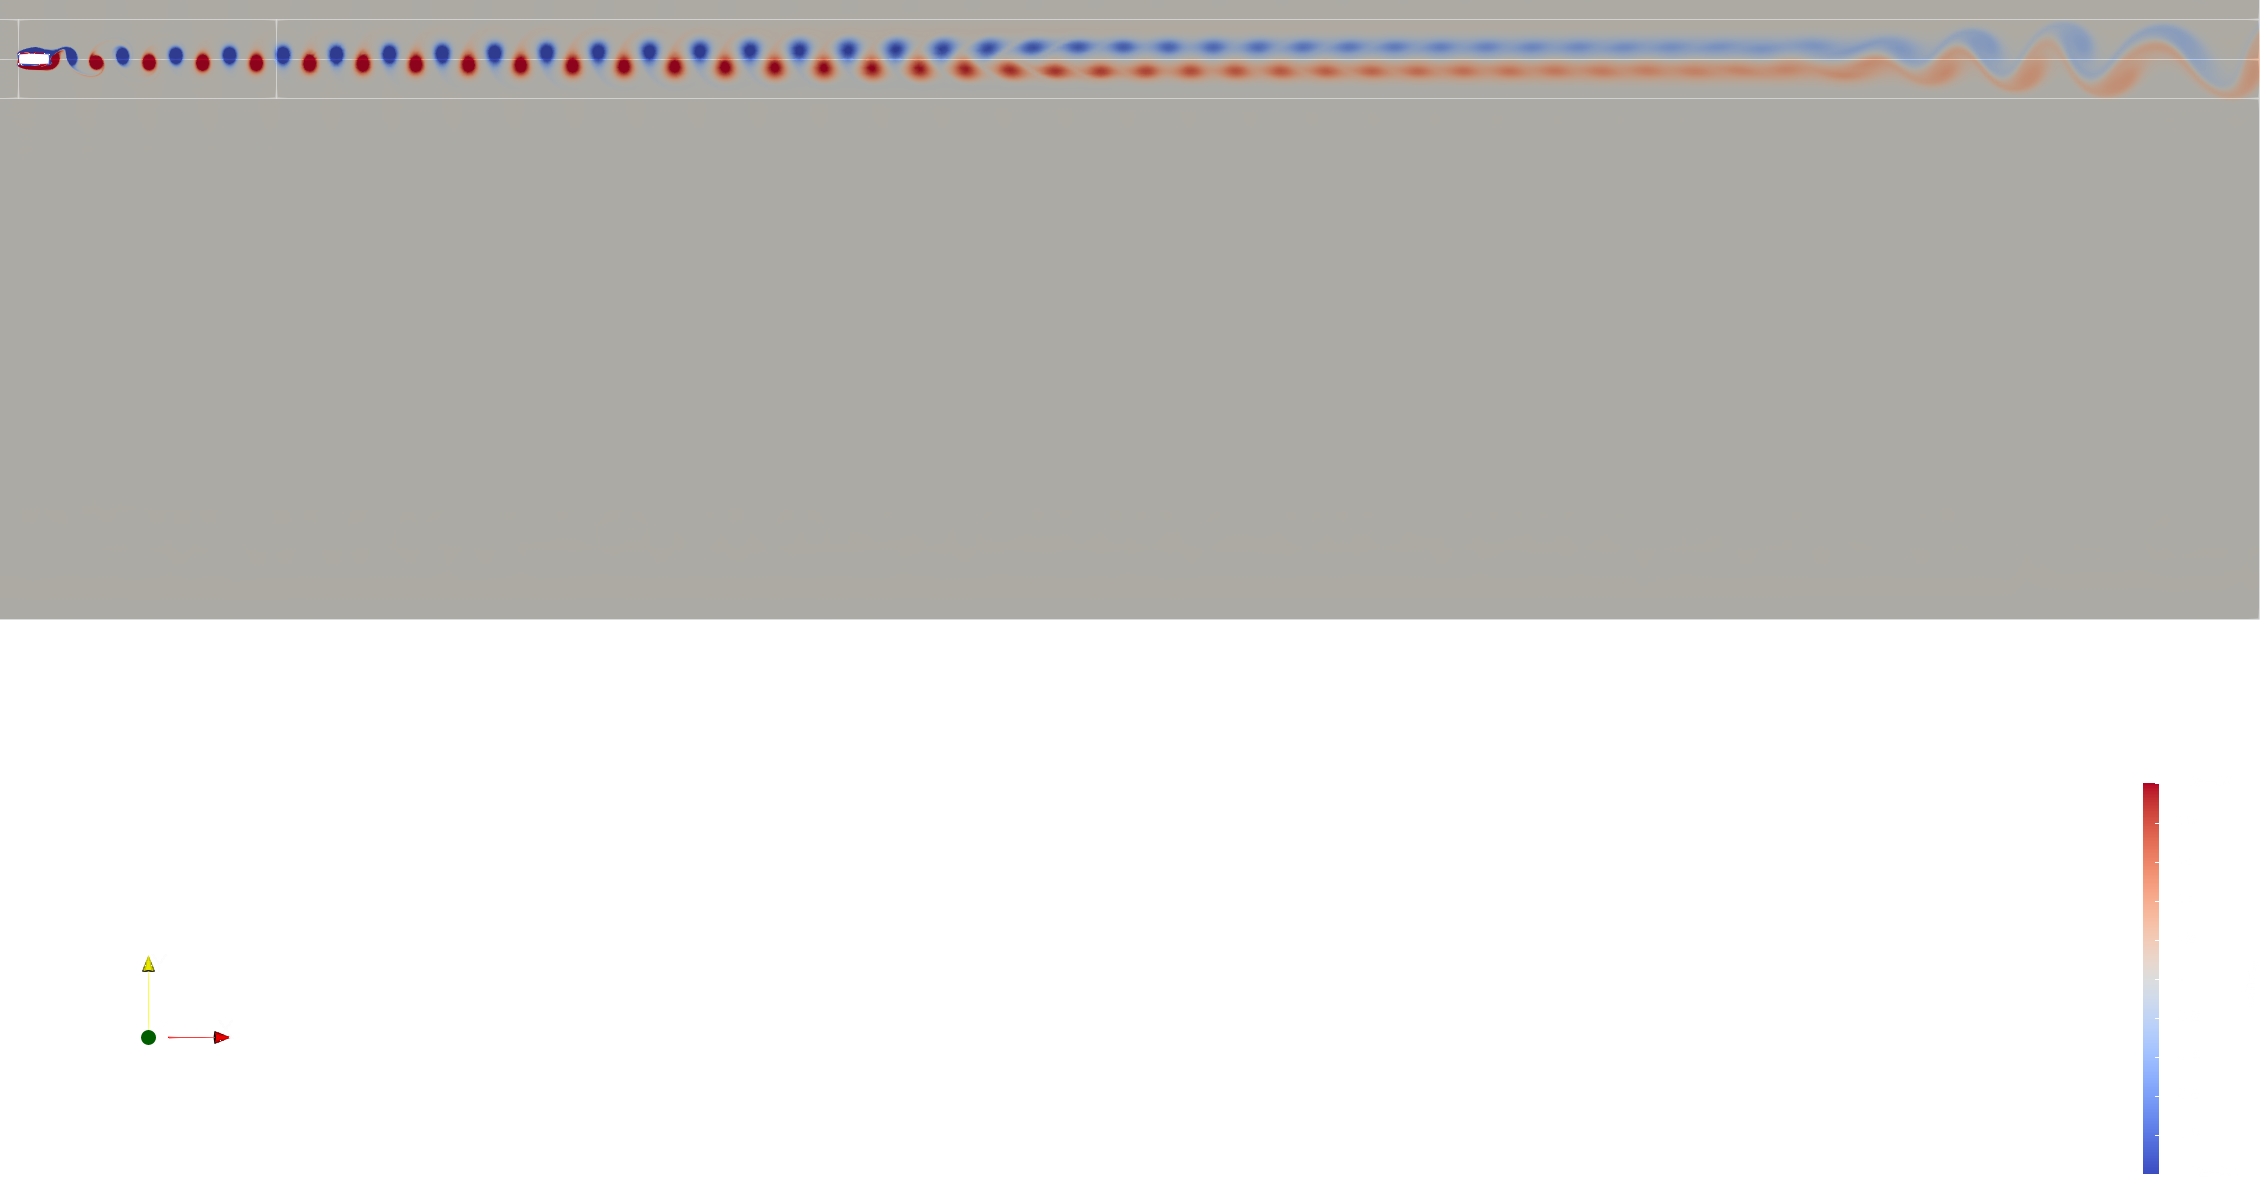
\includegraphics[trim={0 1060 0 0},clip,width=\textwidth]{./fig/appendix/AR2p75_Re450.png}
  %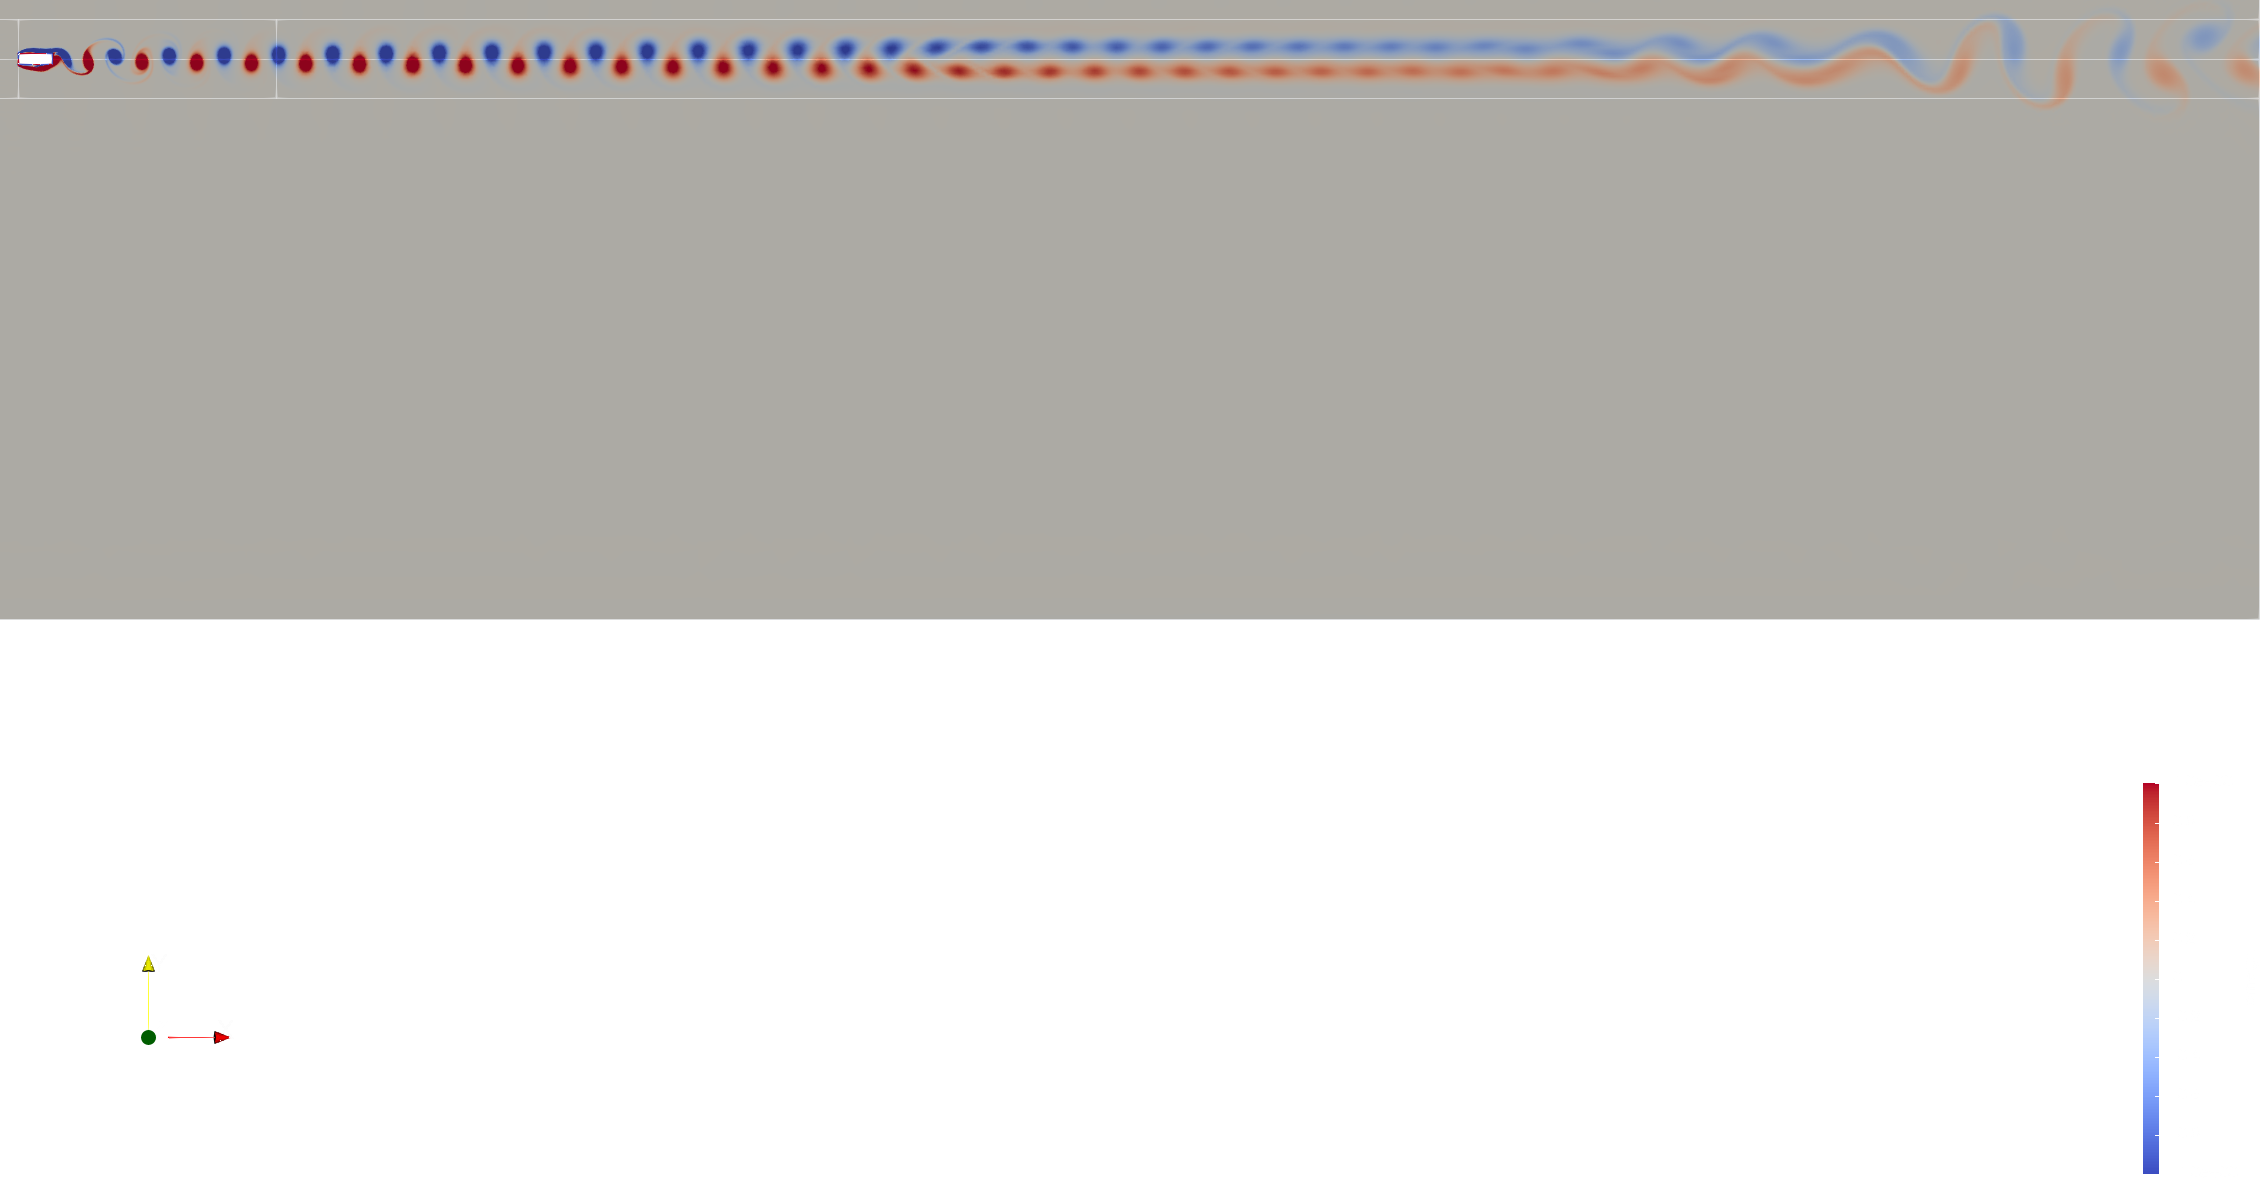
\includegraphics[trim={0 1060 0 0},clip,width=\textwidth]{./fig/appendix/AR3_Re450.png}
  %\vspace{0.5cm}
  %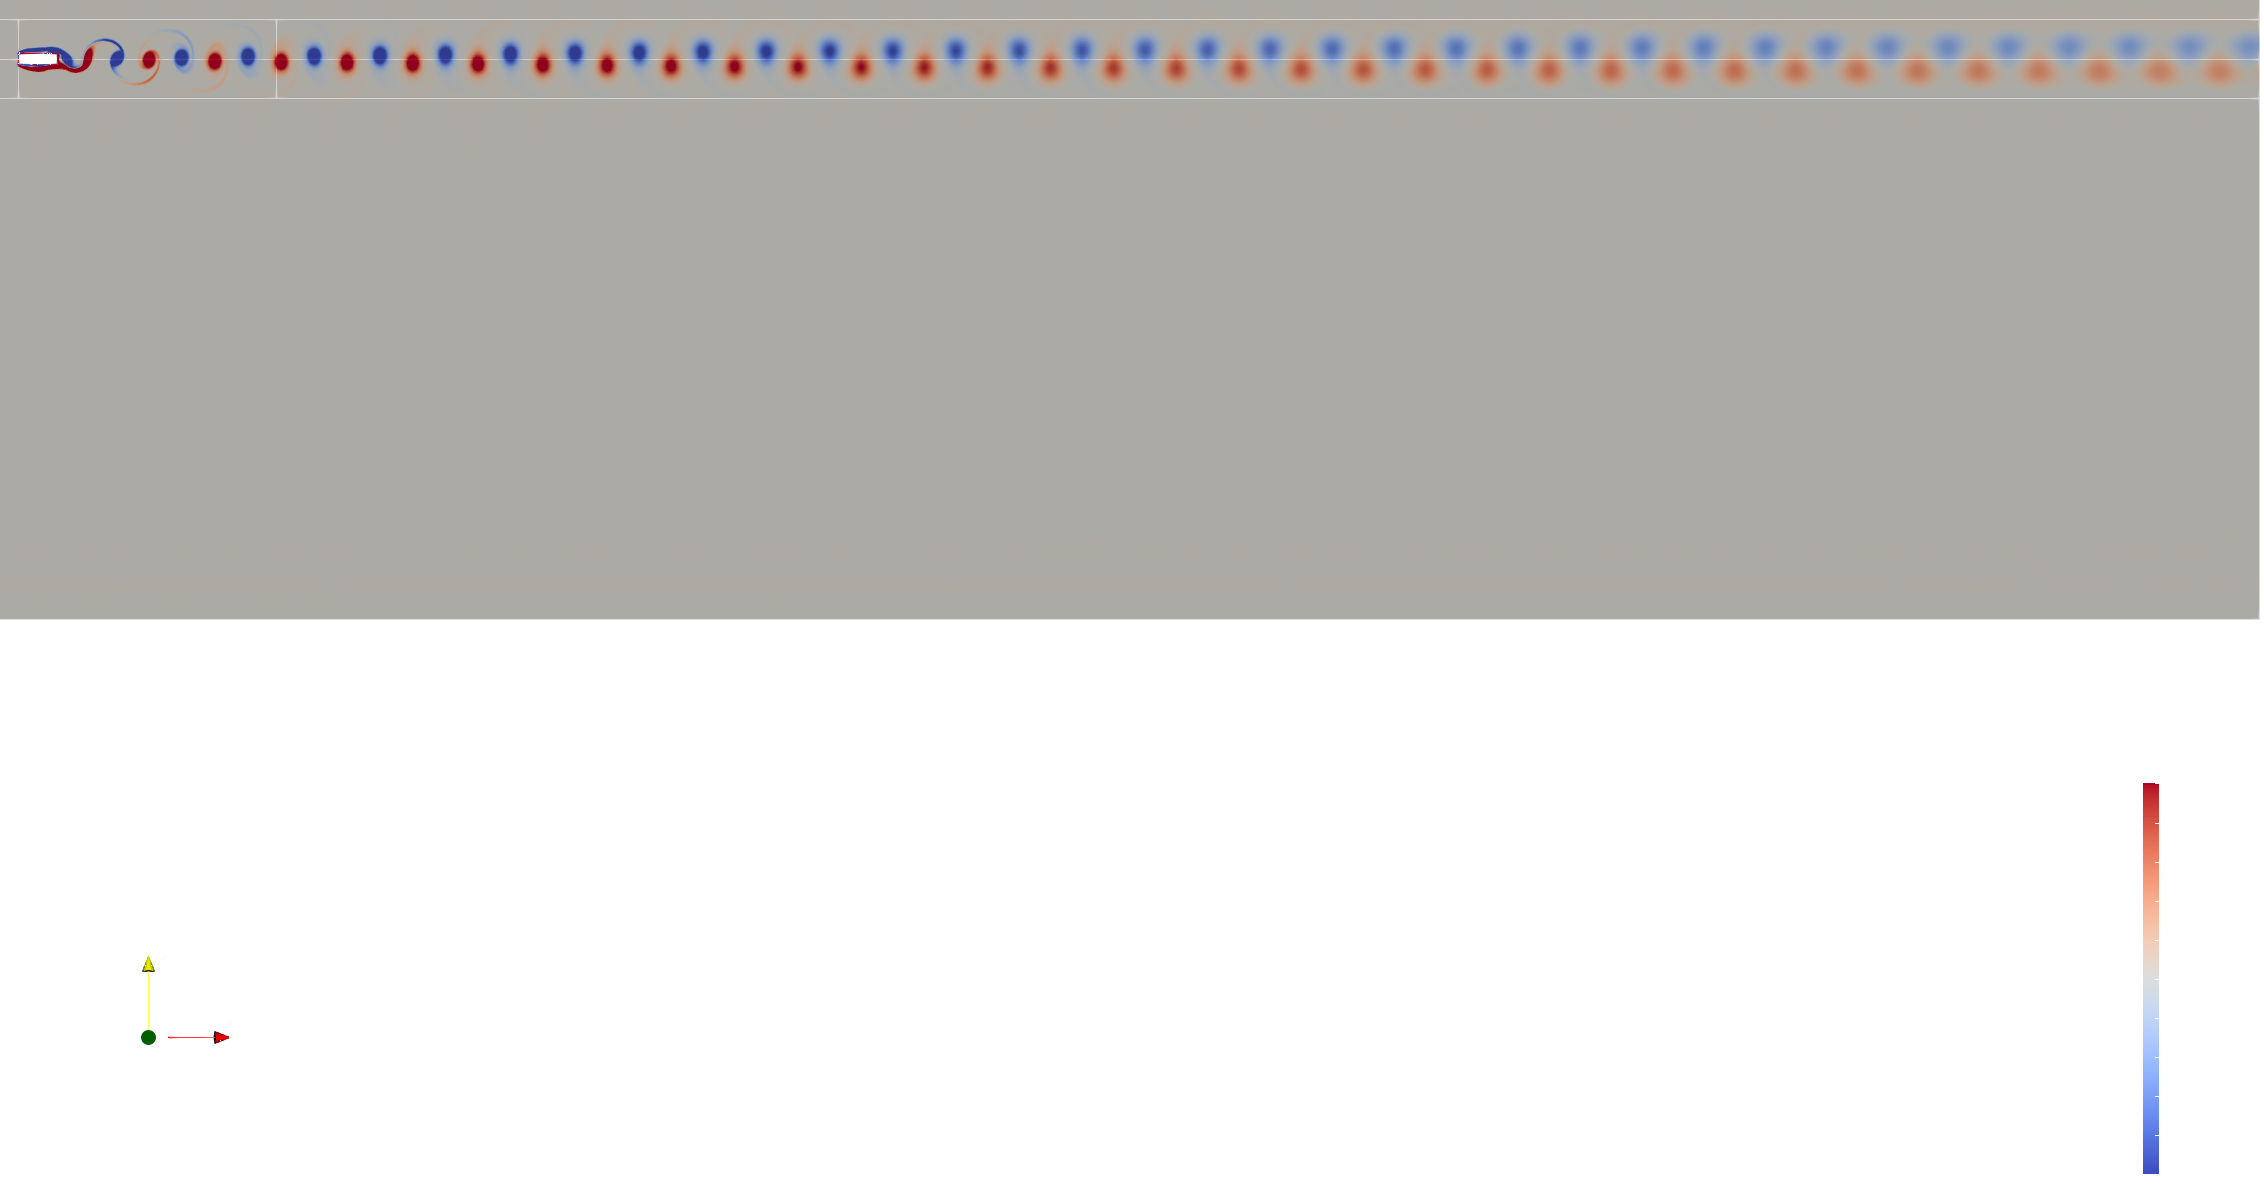
\includegraphics[trim={0 1060 0 0},clip,width=\textwidth]{./fig/appendix/AR3p5_Re450.png}
  %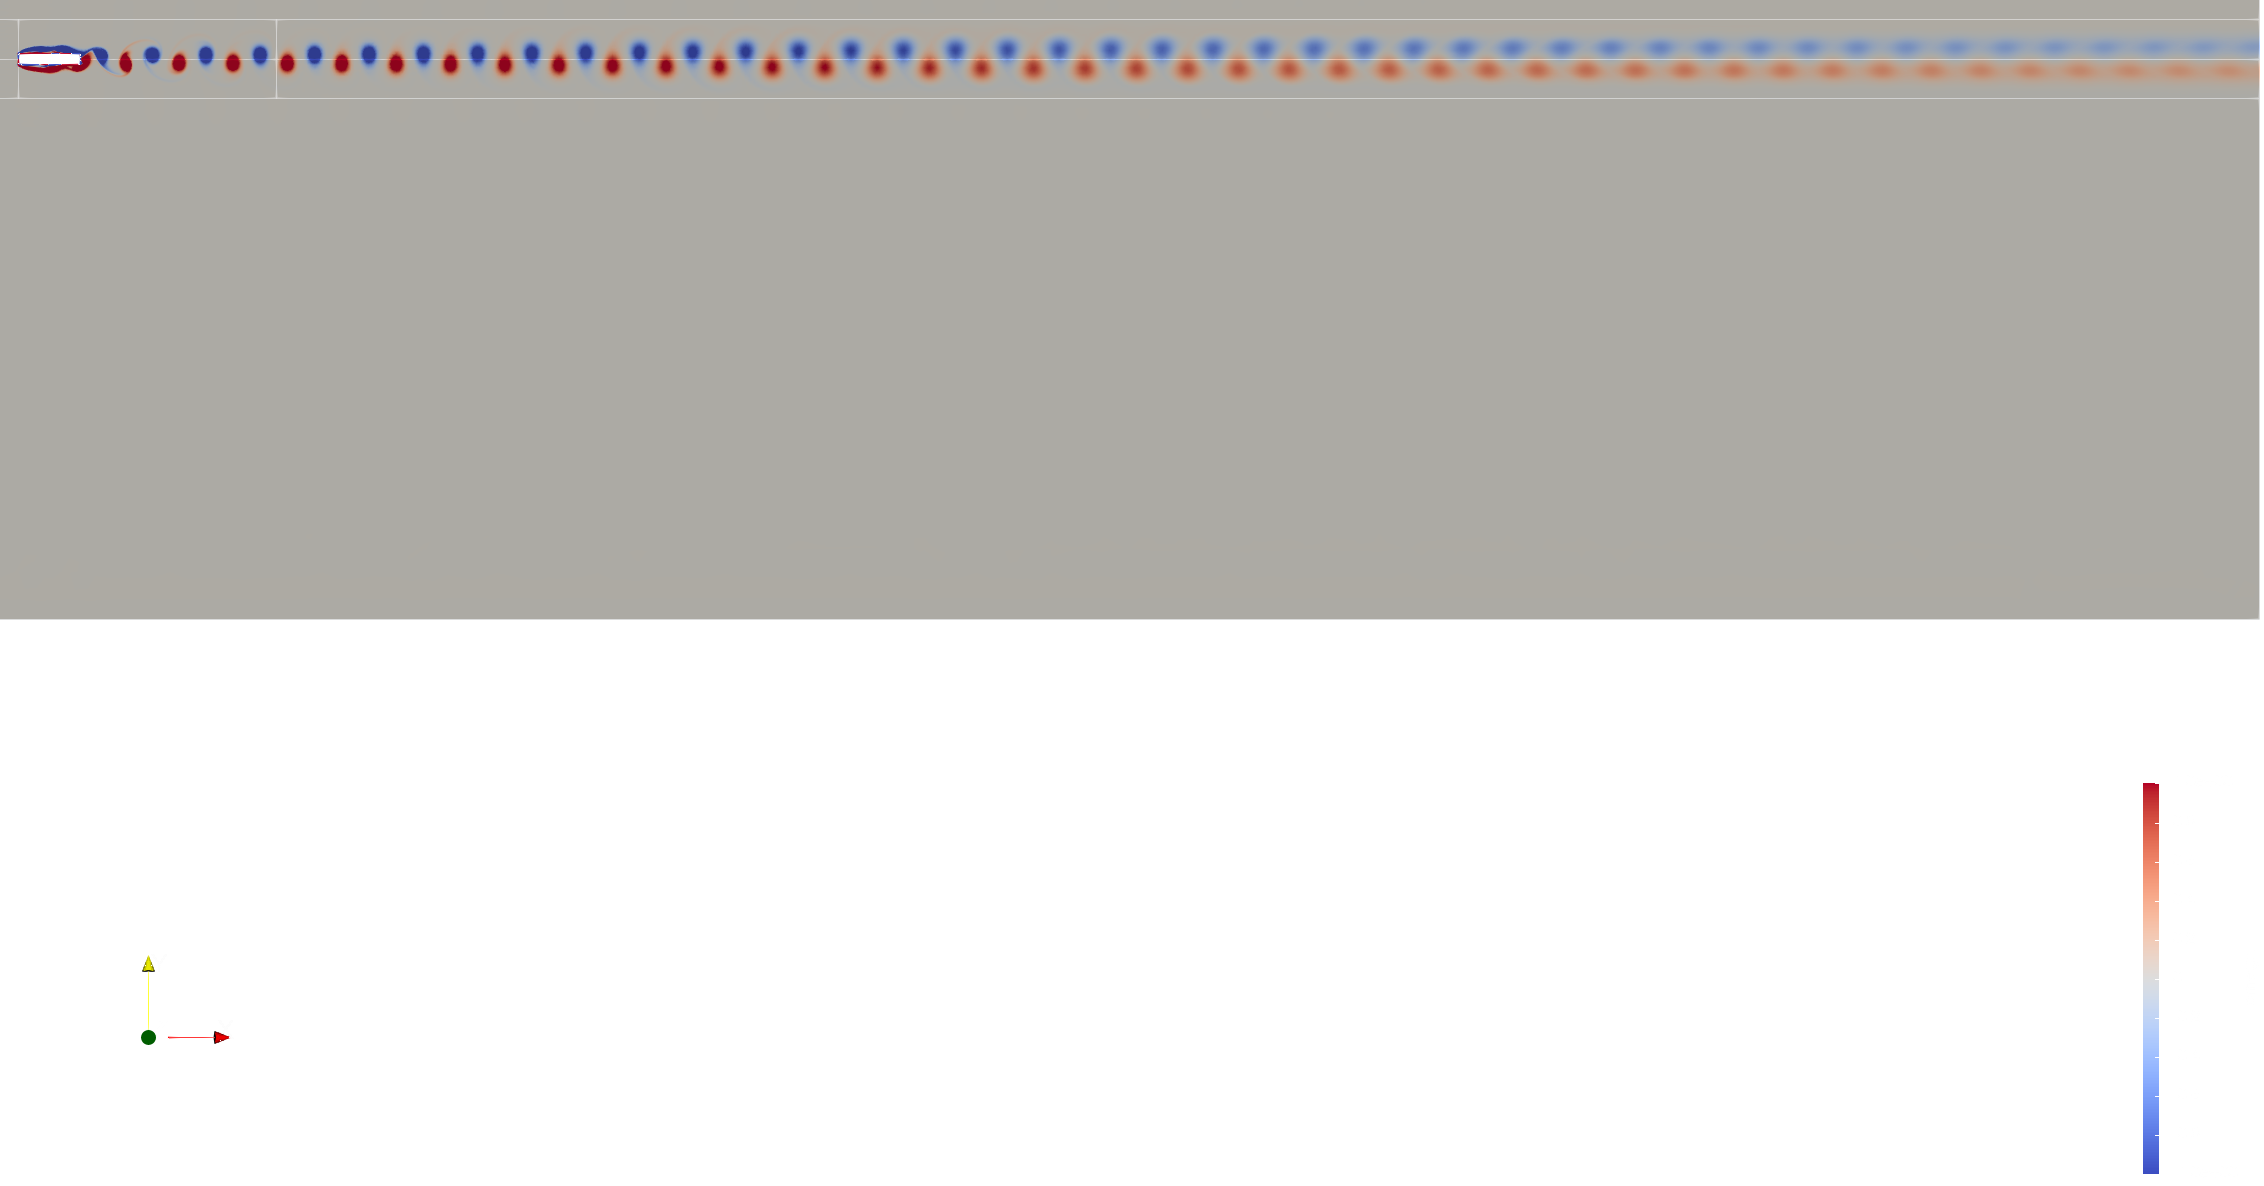
\includegraphics[trim={0 1060 0 0},clip,width=\textwidth]{./fig/appendix/AR5p5_Re450.png}
  %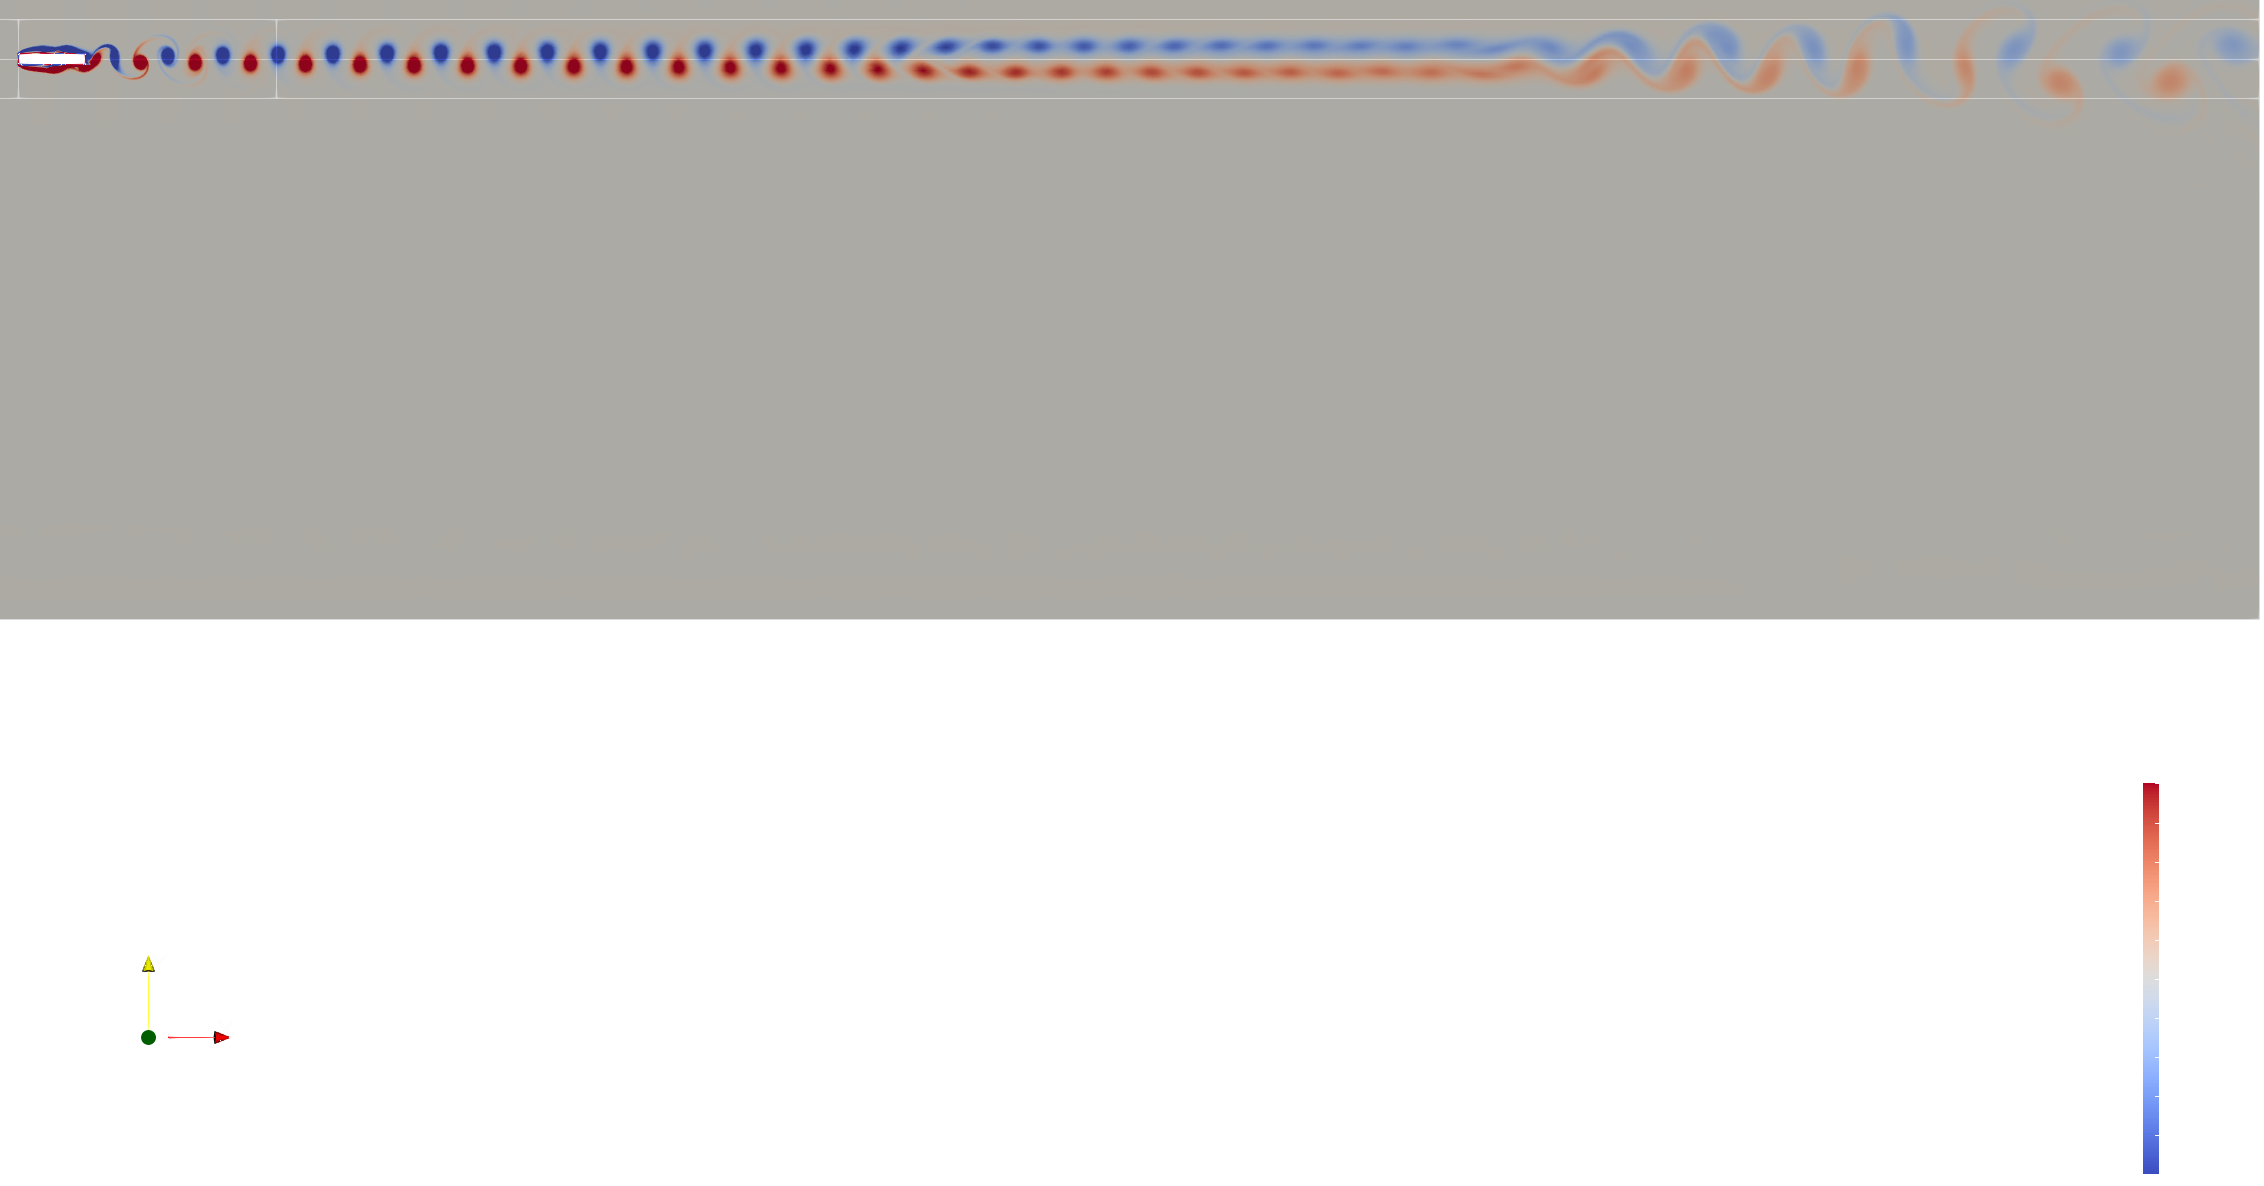
\includegraphics[trim={0 1060 0 0},clip,width=\textwidth]{./fig/appendix/AR6_Re450.png}    
  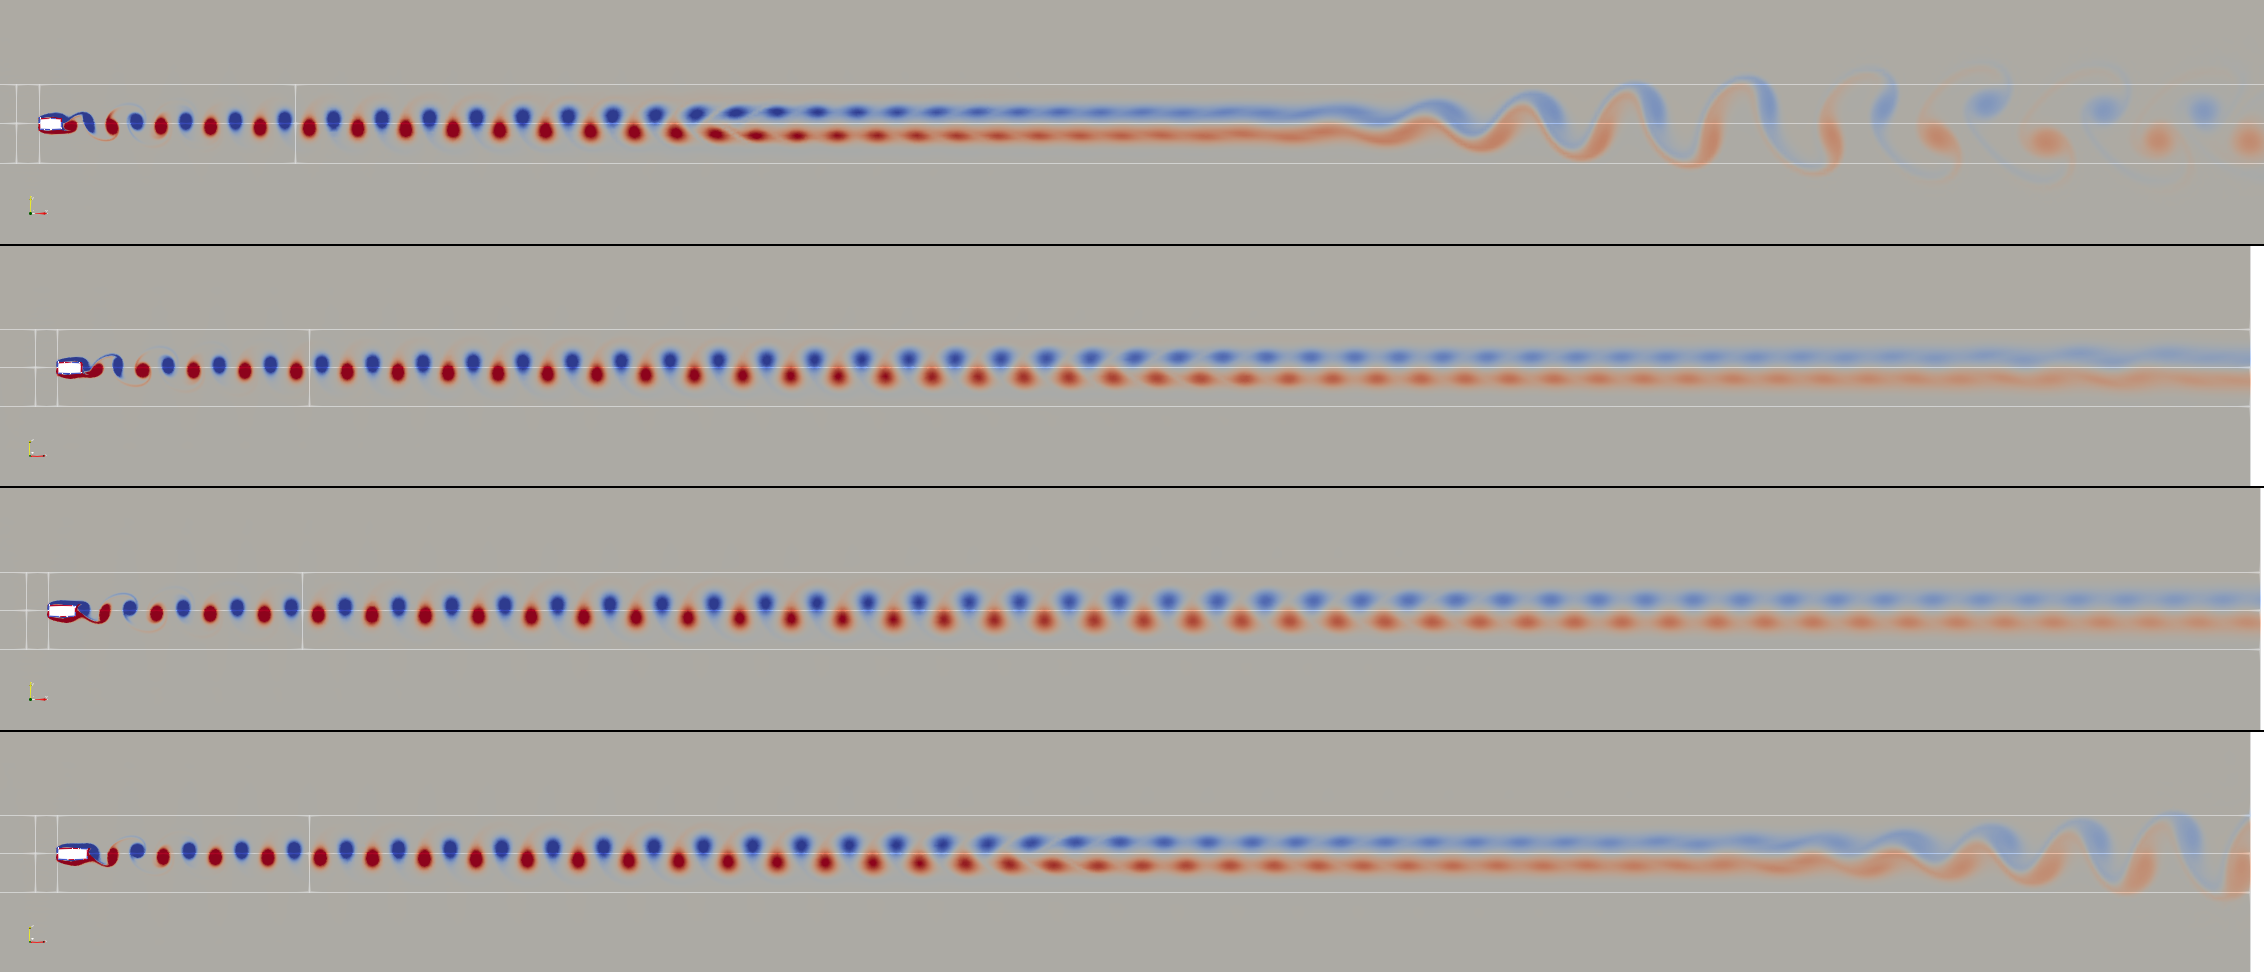
\includegraphics[width=\textwidth]{./fig/appendix/AR_2_2p75_Re450.png}
  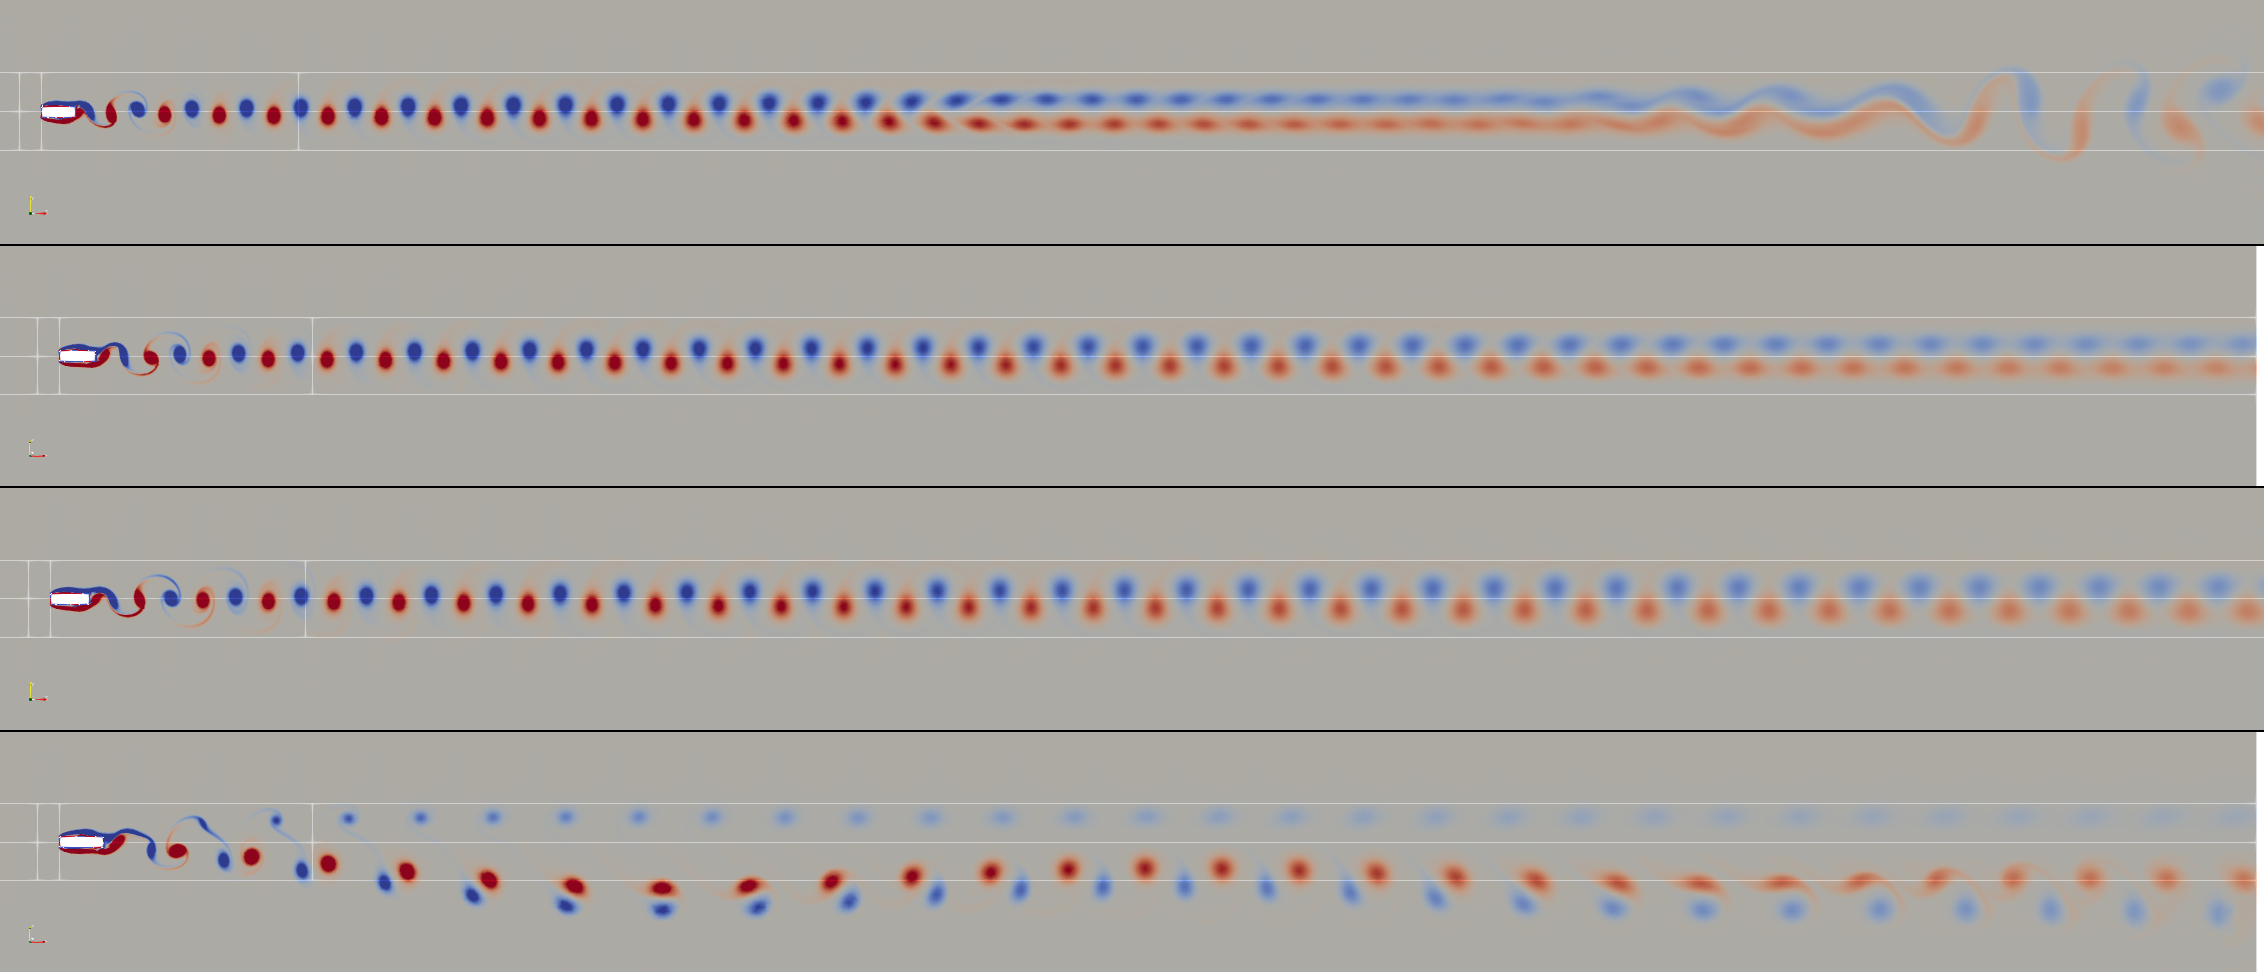
\includegraphics[width=\textwidth]{./fig/appendix/AR_3_4_Re450.png}
  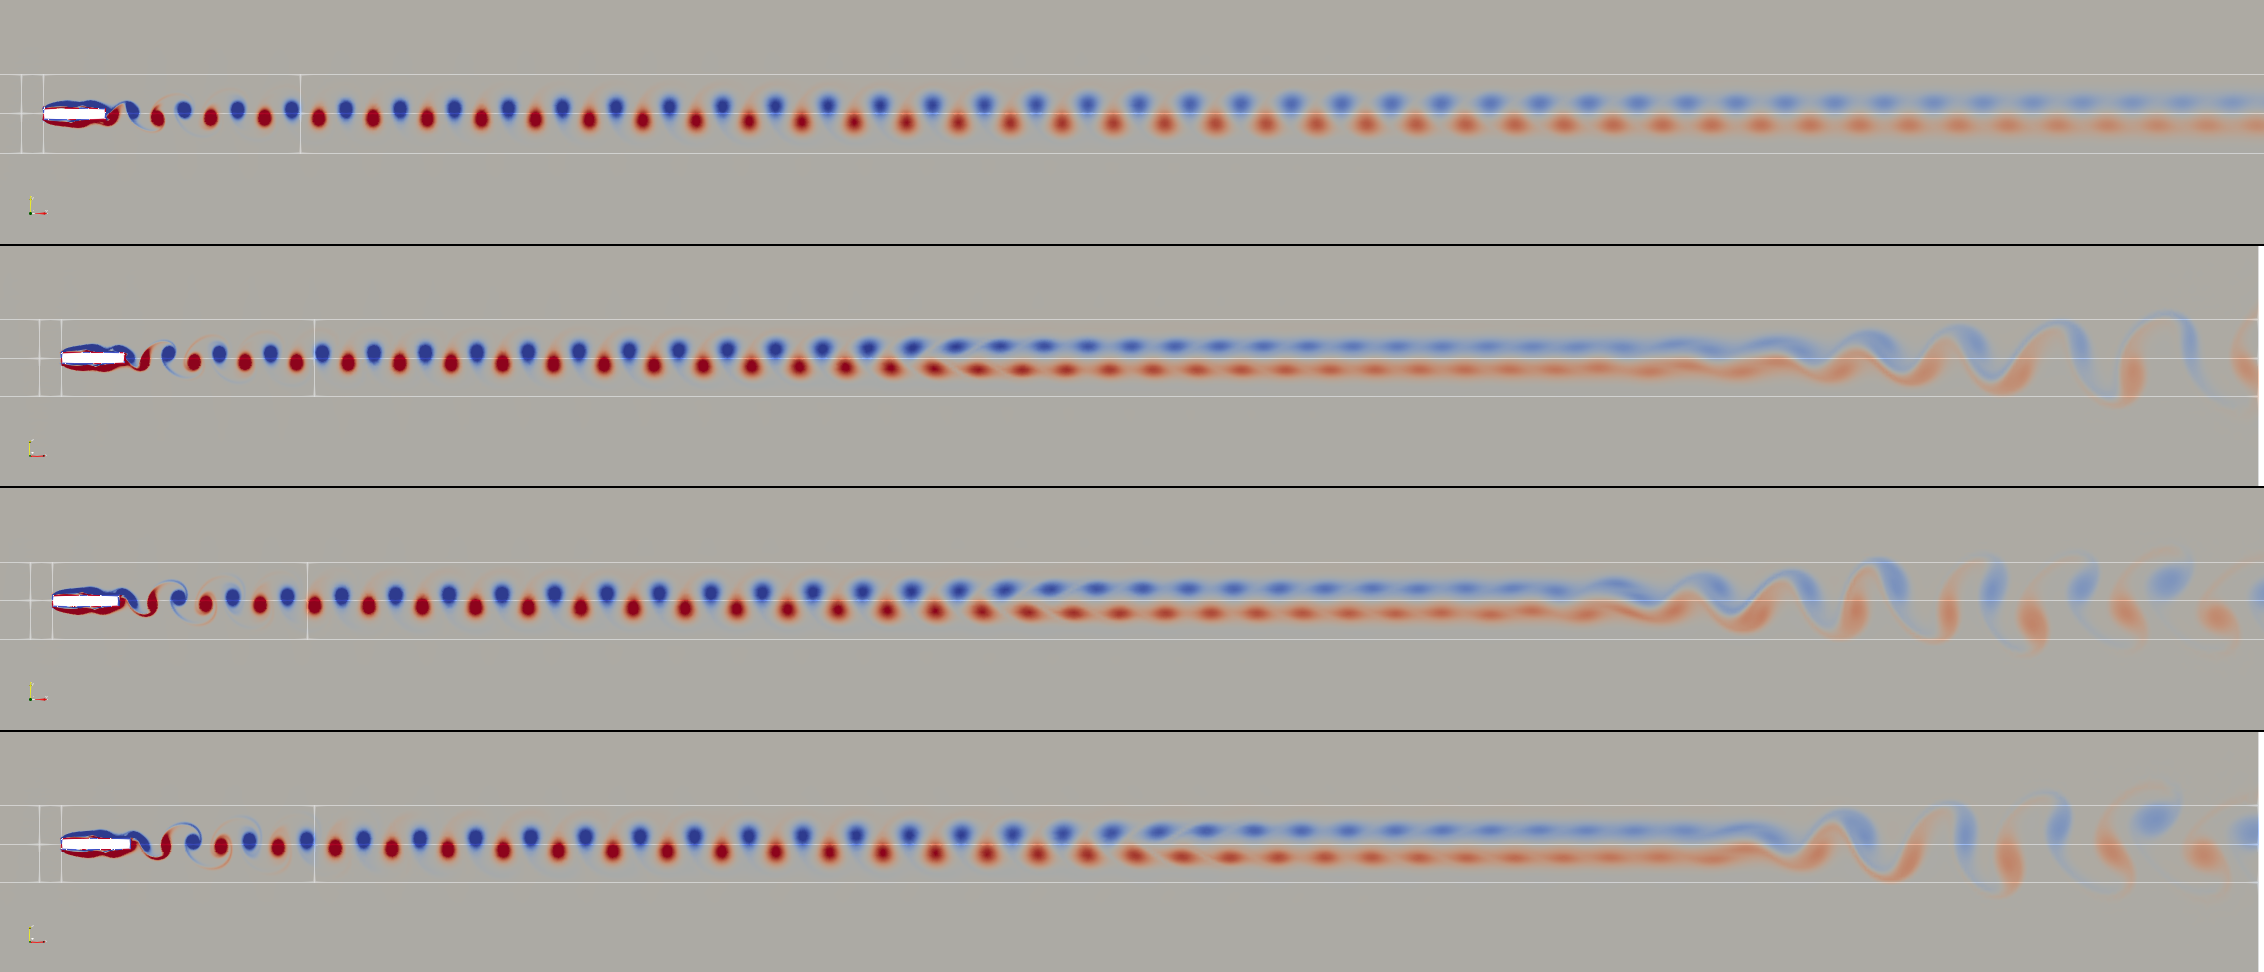
\includegraphics[width=\textwidth]{./fig/appendix/AR_5p5_6p25_Re450.png}    
  \caption{Instantaneous visualisations of the far wake at $Re=450$ for $\AR=2,2.25,2.5,2.75$ (top), $\AR= 3, 3.25, 3.5, 4$ (centre) and $\AR=5.5,5.75,6,6.25$ (bottom). The transition to the two-layered vortex steet and the sucessive transition to the secondary vortex street occurs at different streamwise positions depending of $\AR$. It seems that the transition moves upstream as $\AR$ is increased towards the end of the oblique brach, i.e. towards the point where the TE vortex shedding is permitted. In the case where the flow dynamics is governed by the LE vortex shedding we have that the transition is instead moved downstream. The vortex interaction in the primary vortex street is such that the transition is delayed. We have to verify the $h/a$ threshold to compared with the theory. XX CHECK THE FREQUENCY AT THE DIFFERENT STATIONS. ADD ALSO OTHER $\AR$s. \textcolor{red}{DO WE WANT THE AVERAGE FIELD, WITHOUT WE CAN NOT DO SEVERAL THINGS} XX}
  \label{fig:wake}
\end{figure}

\begin{figure}
\centering
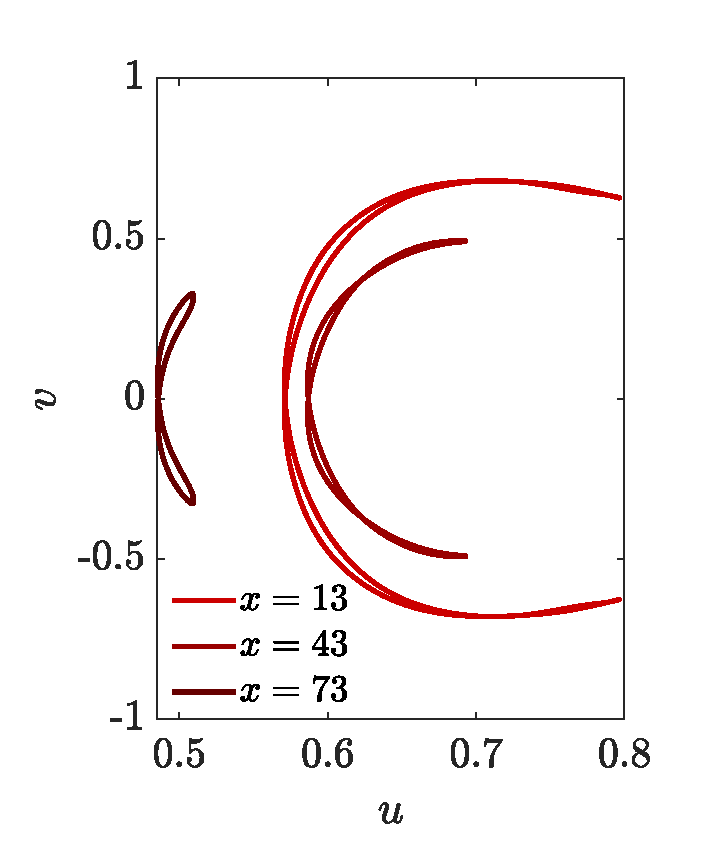
\includegraphics[width=0.328\textwidth]{./fig/appendix/uv_xw_AR3_Re450_a.eps}
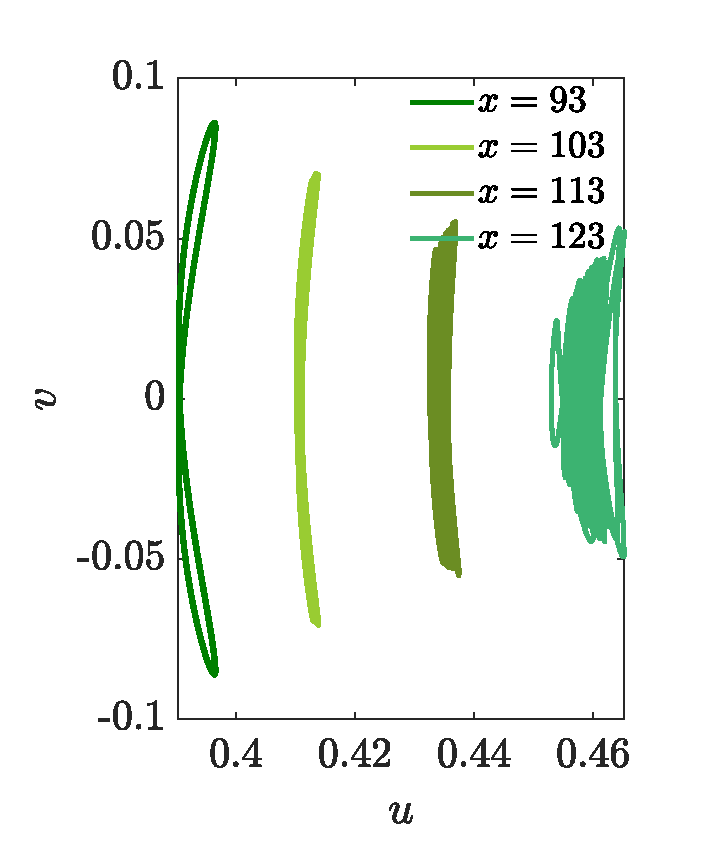
\includegraphics[width=0.328\textwidth]{./fig/appendix/uv_xw_AR3_Re450_b.eps}
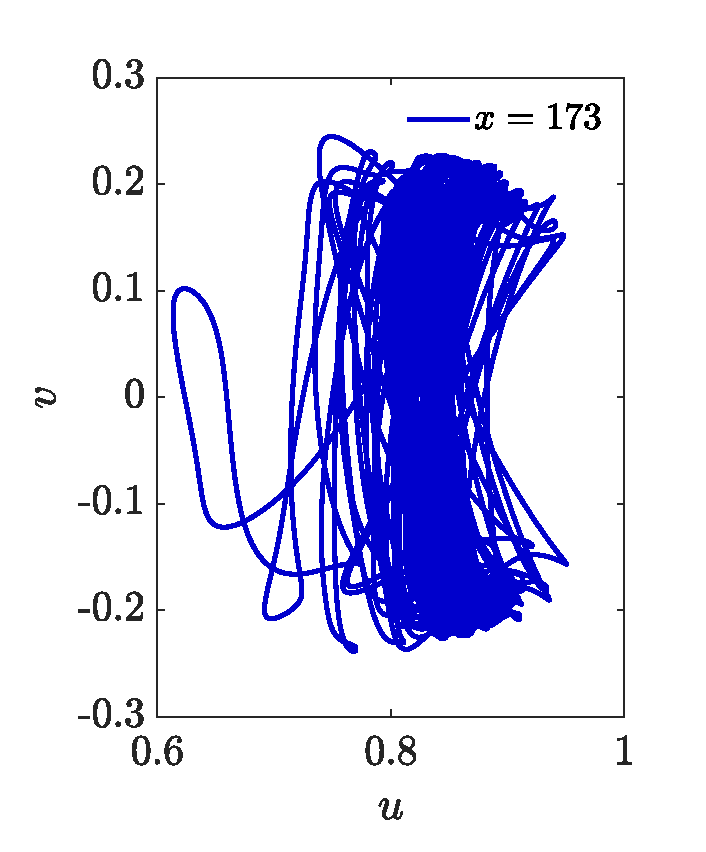
\includegraphics[width=0.328\textwidth]{./fig/appendix/uv_xw_AR3_Re450_c.eps}
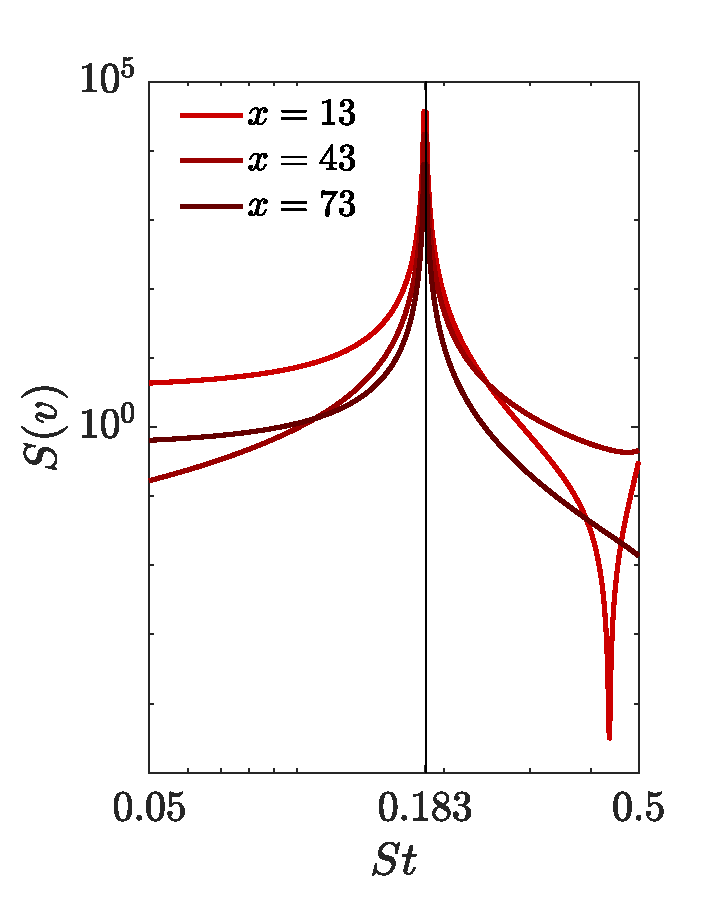
\includegraphics[width=0.328\textwidth]{./fig/appendix/Spec_AR3_Re450_a.eps}
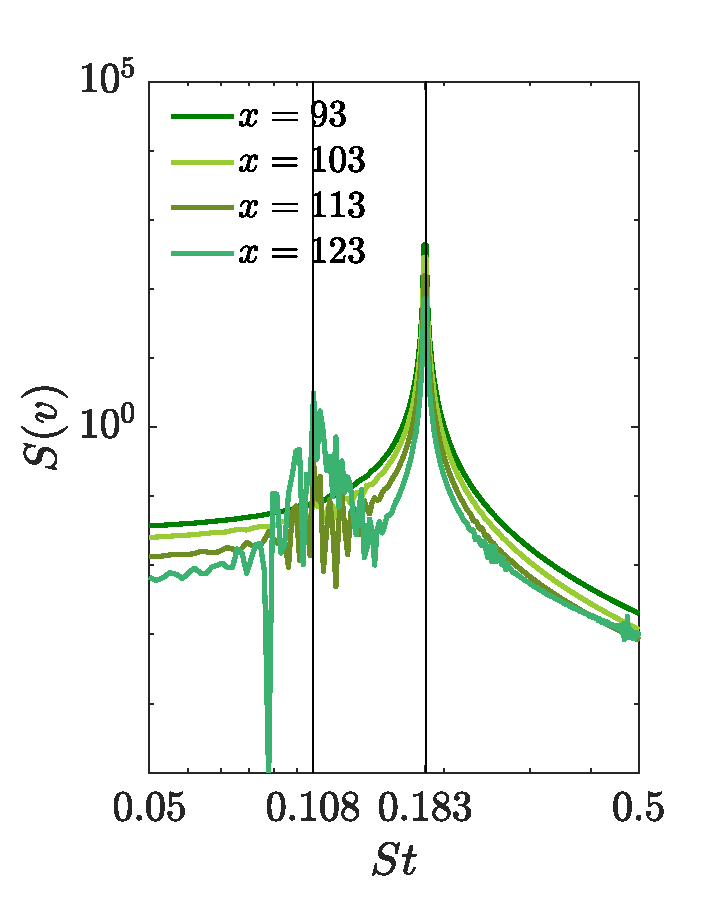
\includegraphics[width=0.328\textwidth]{./fig/appendix/Spec_AR3_Re450_b.eps}
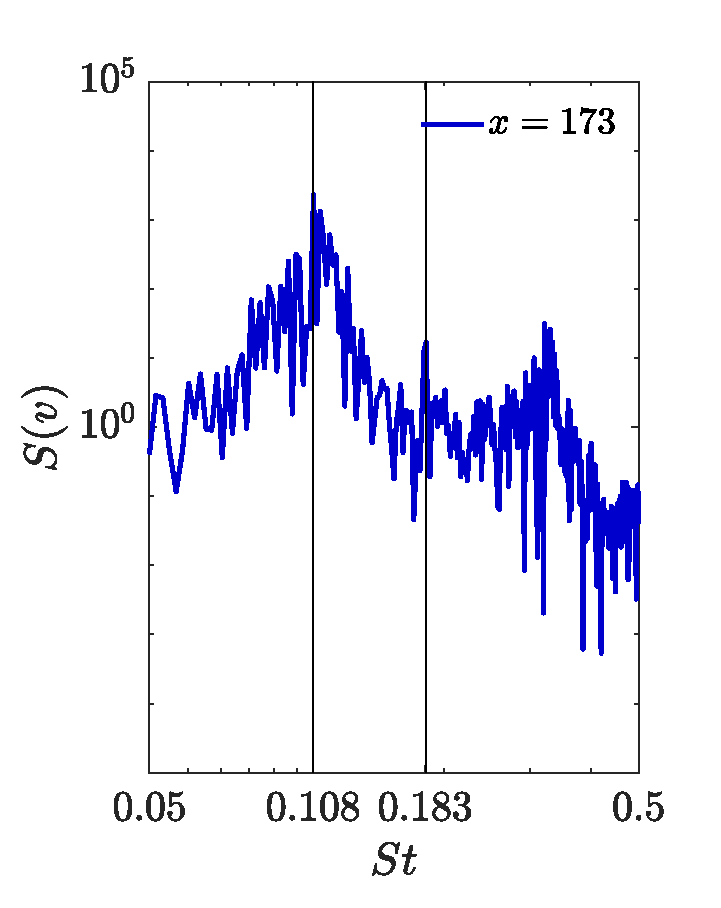
\includegraphics[width=0.328\textwidth]{./fig/appendix/Spec_AR3_Re450_c.eps}
\caption{Phase space diagrams and frequency spectra plots in the wake for $\AR=3$ and $Re=450$. Top: $u-v$ diagrams at different streamwise locations. Bottom: frequency spectra $S(v)$ at different streamwise locations. Left: primary vortex street. Centre: two-layered wake. Right: secondary vortex street.}
\label{fig:wake_AR3}
\end{figure}

\begin{figure}
\centering
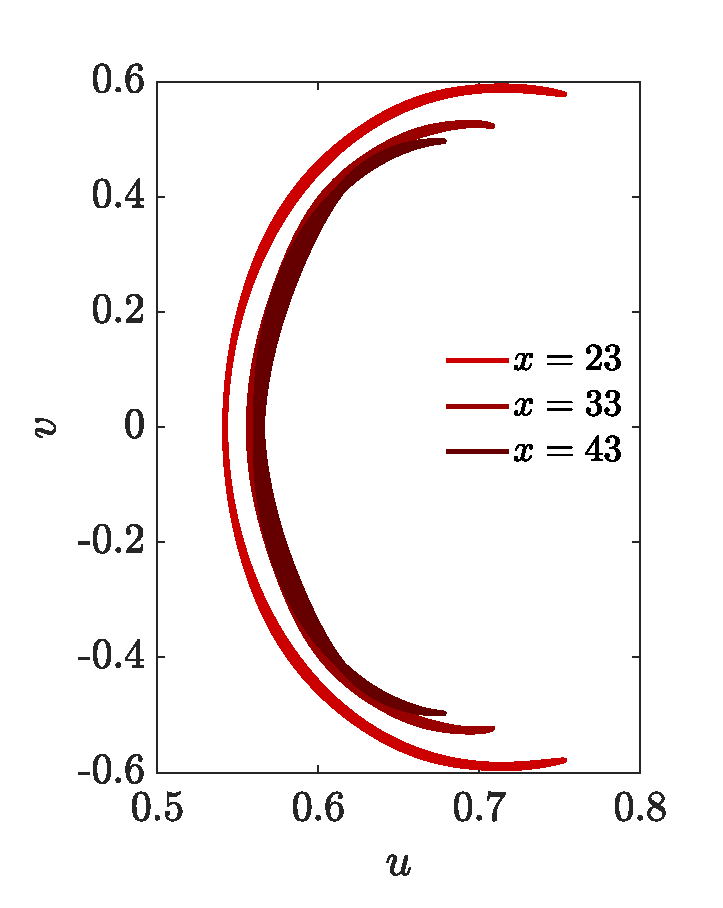
\includegraphics[width=0.328\textwidth]{./fig/appendix/uv_xw_AR6_Re450_a.eps}
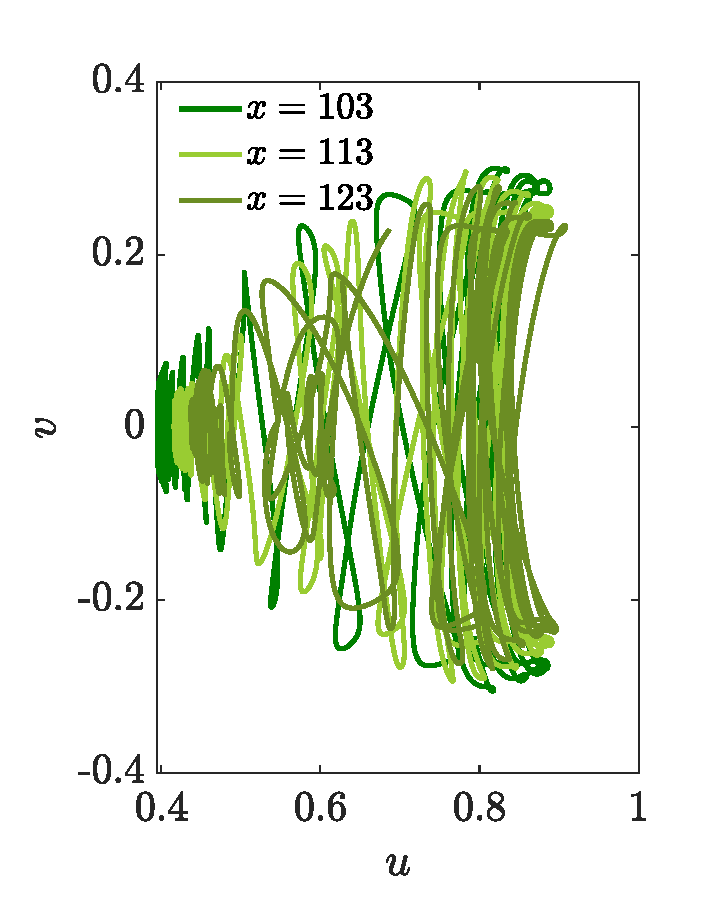
\includegraphics[width=0.328\textwidth]{./fig/appendix/uv_xw_AR6_Re450_b.eps}
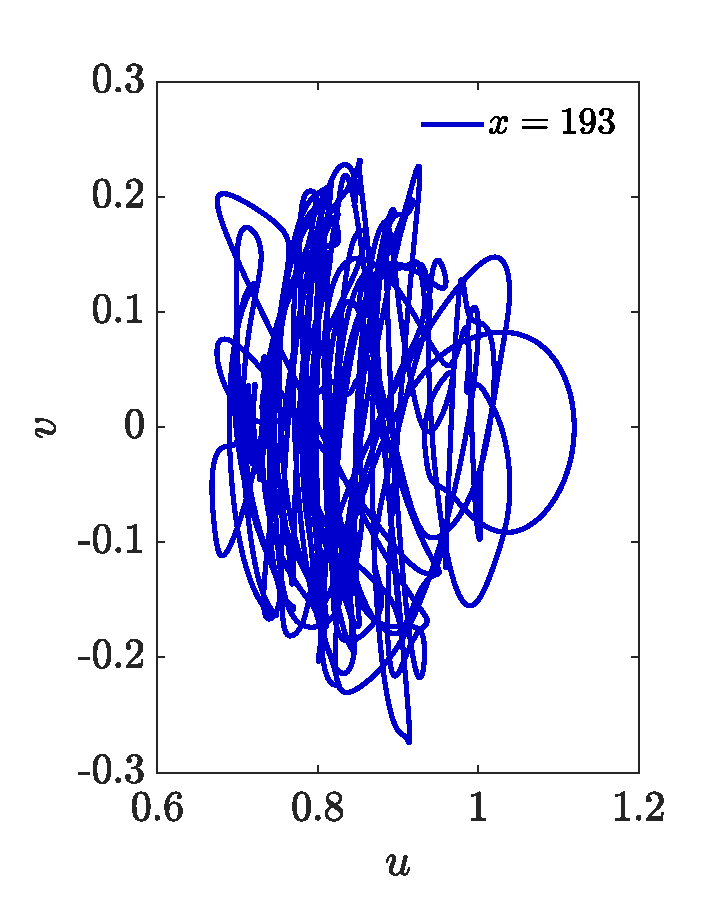
\includegraphics[width=0.328\textwidth]{./fig/appendix/uv_xw_AR6_Re450_c.eps}
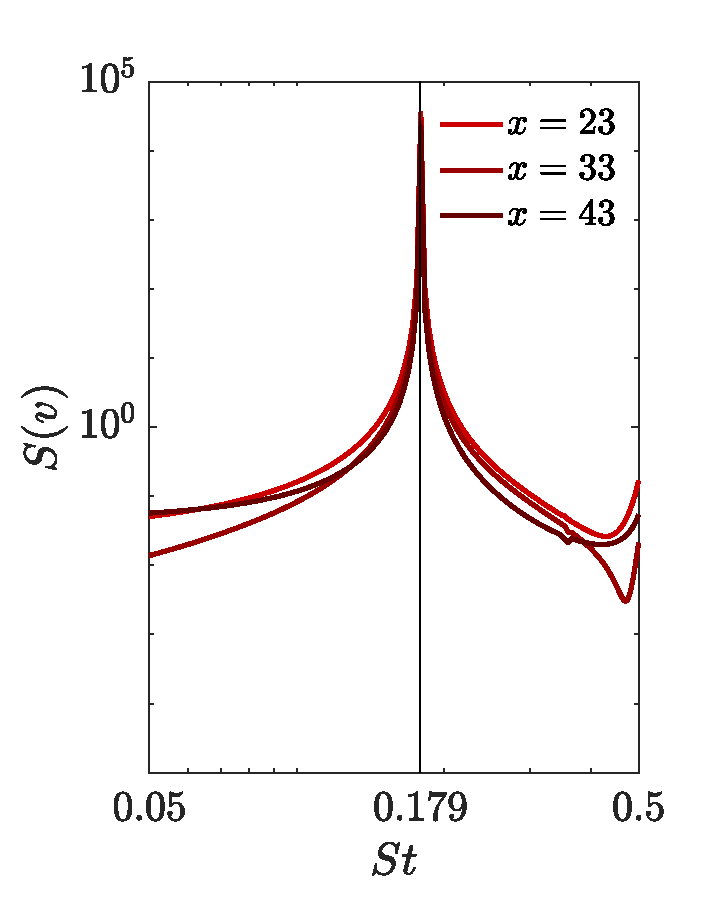
\includegraphics[width=0.328\textwidth]{./fig/appendix/Spec_AR6_Re450_a.eps}
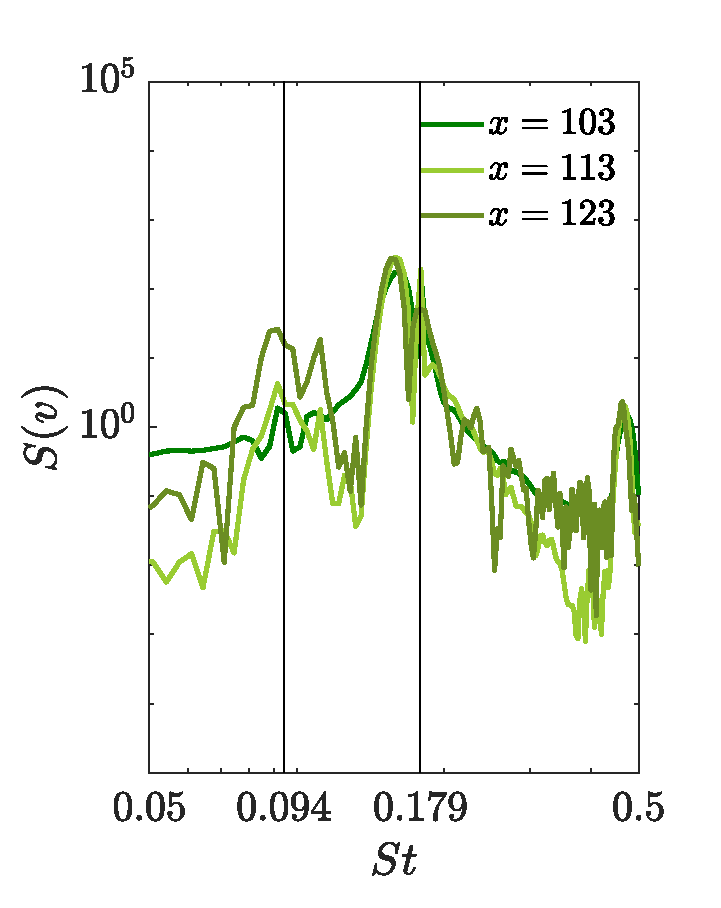
\includegraphics[width=0.328\textwidth]{./fig/appendix/Spec_AR6_Re450_b.eps}
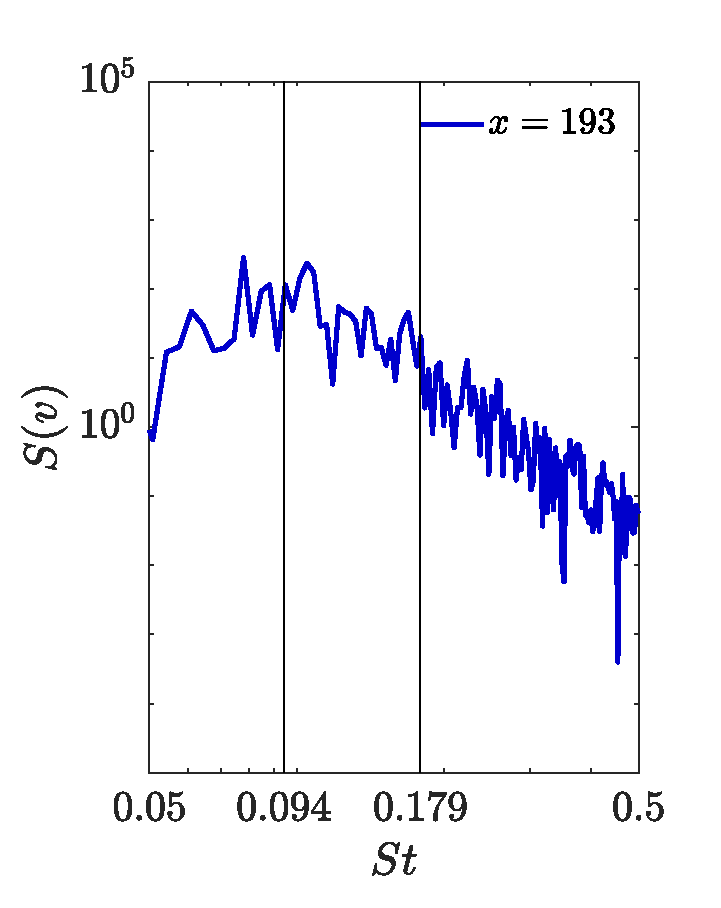
\includegraphics[width=0.328\textwidth]{./fig/appendix/Spec_AR6_Re450_c.eps}
\caption{As figure \ref{fig:wake_AR6}, but for $\AR=6$. XX UPDATE WITH MORE DATA XX.}
\label{fig:wake_AR6}
\end{figure}

We start considering $\AR=3$ at $Re=450$ as an example, see figure \ref{}. The wake flow can be separated into three regimes, namely the primary vortex street, the two layered vortices and the secondary vortex street. Following \cite{jiang-cheng-2019} the streamwise locations of the first and second transitions can be determined by the time-averaged $\langle v \rangle$ field. Indeed, two pairs of local maxima are observed in correspondence of this transition, as here the flow is diverted away from the wake centreline. The second location of local maxima of $\langle v \rangle$, instead, corresponds to the second transition where the flow starts to reoccupy the wake centreline. The distinction between the different flow regimes is evident also when looking at the time-averaged Reynolds shear stresses $\langle u'v' \rangle$. Accordingly, the Reynolds shear stresses are substantially null in the two-layered region, which is commonly referred to as the ``calm region'' \citep{durgin-karlsson-1971}.

We now show the influence of $\AR$. Here the focus in of $\AR \ge 2.5$ and fix the Reynolds number to $Re=450$. Results for $4 \le \AR 4.5$ are not reproted, as here at this $Re$ the near wake undergoes a two-dimensional instability which leads to a slanted wake. In this case the two-layered wake and the secondary vortex street are not observed. \textcolor{red}{XX Dependence of the position of the two transitions points on $\AR$ at this $Re$, explain how this changes with the near-wake flow topology XX}

Figure \ref{} shows the frequency spectra of the time histories of $v$ sampled at $y=0$ and various $x$ positions for different $\AR$s. \textcolor{red}{XX Figure with different pannels. For each panel we show the frequency spectra at different $x$ positions for different $\AR$s XX}We look at the spectra of $u_y$. Accordinlgly, two peaks $f_1$ and $f_2$ are observed in the spectra. The first is well defined and represents the primary vortex shedding frequency. The second peak, instead, consist of a sharp peak together with small-scale broad-band frequencies and is associated with the development of the secondary vortex street. This is clearly shown in figure \ref{}, where the $v$ time signal is shown at two different streamise locations dominated by primary and secondary vortex street. \textcolor{red}{XX Add (i) dependence of $f_1$ and $f_2$ on $x$ and $\AR$, (ii) dependence on $x$ of the intensity of the two peaks for different $\AR$s}.

\textcolor{red}{Do we plot also the evolution of the wake deficit for the different cases? $(1-\langle u \rangle/U_\infty)$}

\cite{durgin-karlsson-1971}, \cite{tsuboi-oshima-1985} and \cite{karasudani-funakoshi-1994} investigated the stability of the geoemtrical arrangement of vortices in a wake shown that when the spacing ratio $h/a$ was larger that $0.365$, the vortices would rotate to align with the streamwise direction and stretch out and diffuse resulting into a near-parallel shear flow. When this flors, the near-stationaly wake is convectively unstable and may form a new secondary vortex street with a longer wavelenght and a lower frequency. This has been investigated also by \cite{thompson-etal-2014} in the context of the flow past two-dimensional elliptic bluff bodies. Figure \ref{} shows the variation of the spacing ration with downstream distance for a number of different $\AR$s. \textcolor{red}{XX Comment on what we observed and the streamwise location at which we observe that the ratio becomes larger than the threshold. Relate this with the above discussion XX}


\textcolor{red}{We can perfrom DMD analysis of the far wake. Look at \cite{thompson-etal-2014}.}


\iffalse

\begin{figure}
  \centering
  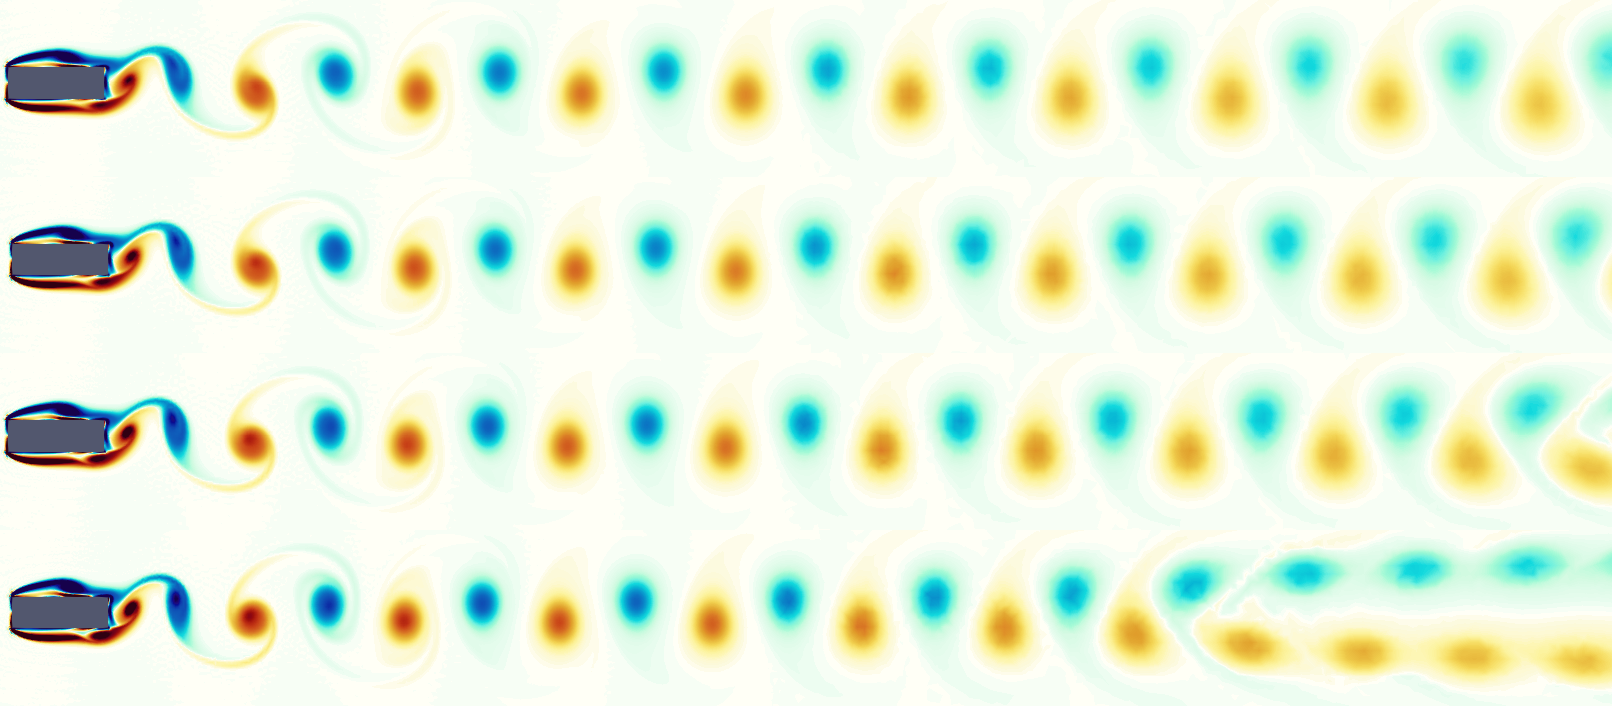
\includegraphics[width=0.8\textwidth]{./fig/AR3/BF_vort_Re400_475.png}
  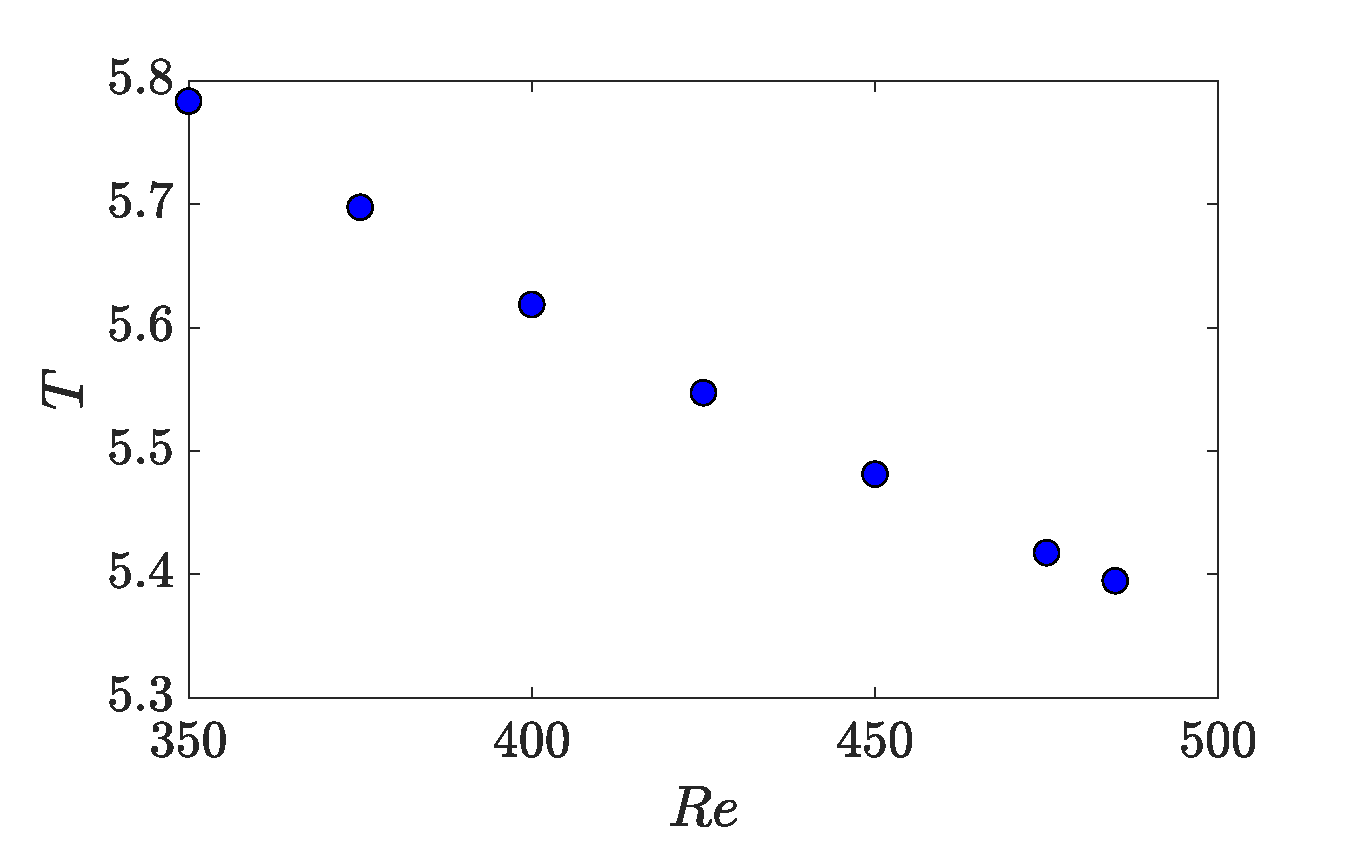
\includegraphics[width=0.5\textwidth]{./fig/AR3/T_Re.eps}
  \caption{Base flow vorticity snapshots for $\AR=3$ at (from top to bottom) $Re=400$, $Re=425$, $Re=450$ and $Re=485$. Note that as $Re$ increases the structure of the wake changes, with the positive and negative vorticity monopoles being clearly separated. As $Re$ increases, this separation start occurring closer to the TE. Bottom panel: Dependence of the period $T$ on $Re$ for the periodic regime in the $350 \le Re \le 485$ range.}
  \label{fig:BF_AR3}
\end{figure}

\begin{figure}
  \centering
  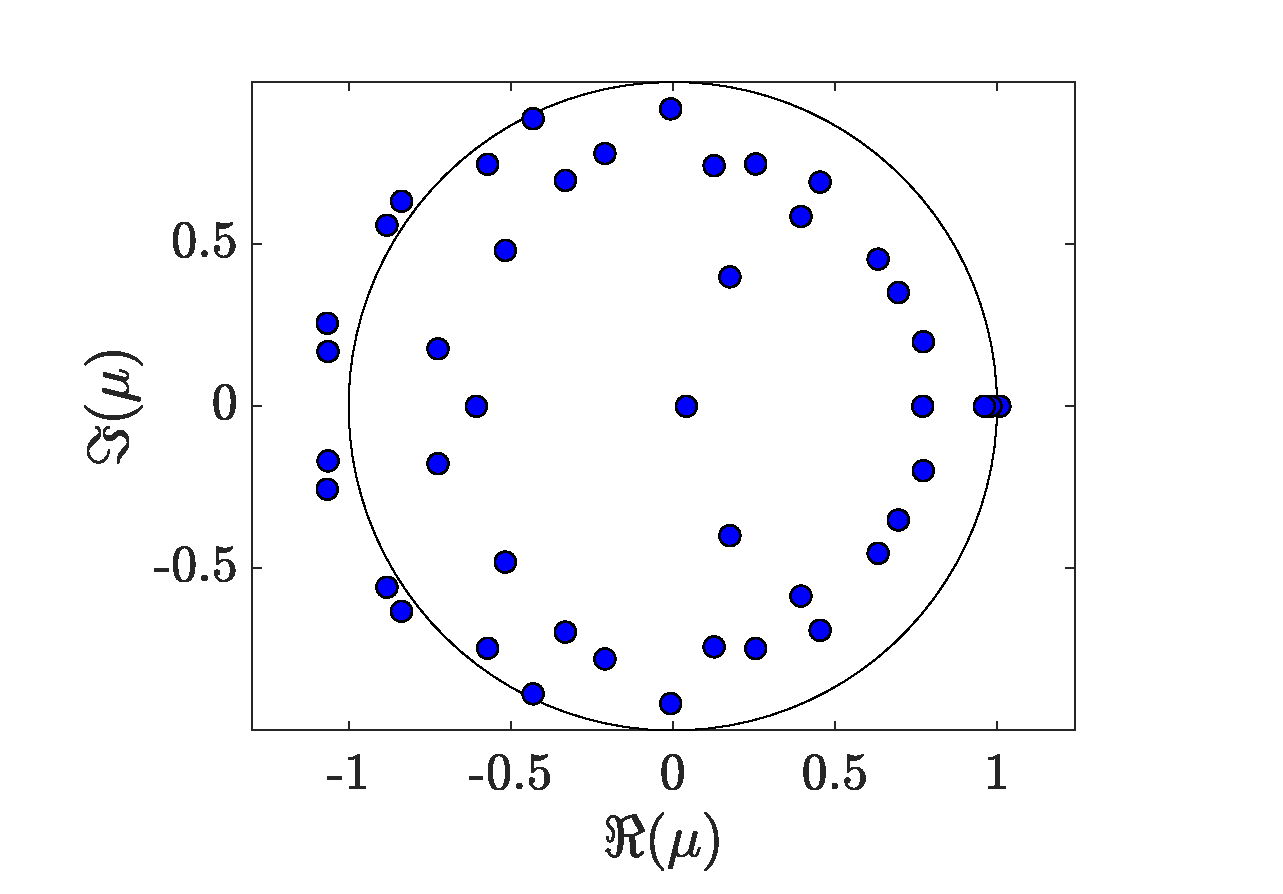
\includegraphics[width=0.5\textwidth]{./fig/AR3/mult_Re495_beta0.eps}
  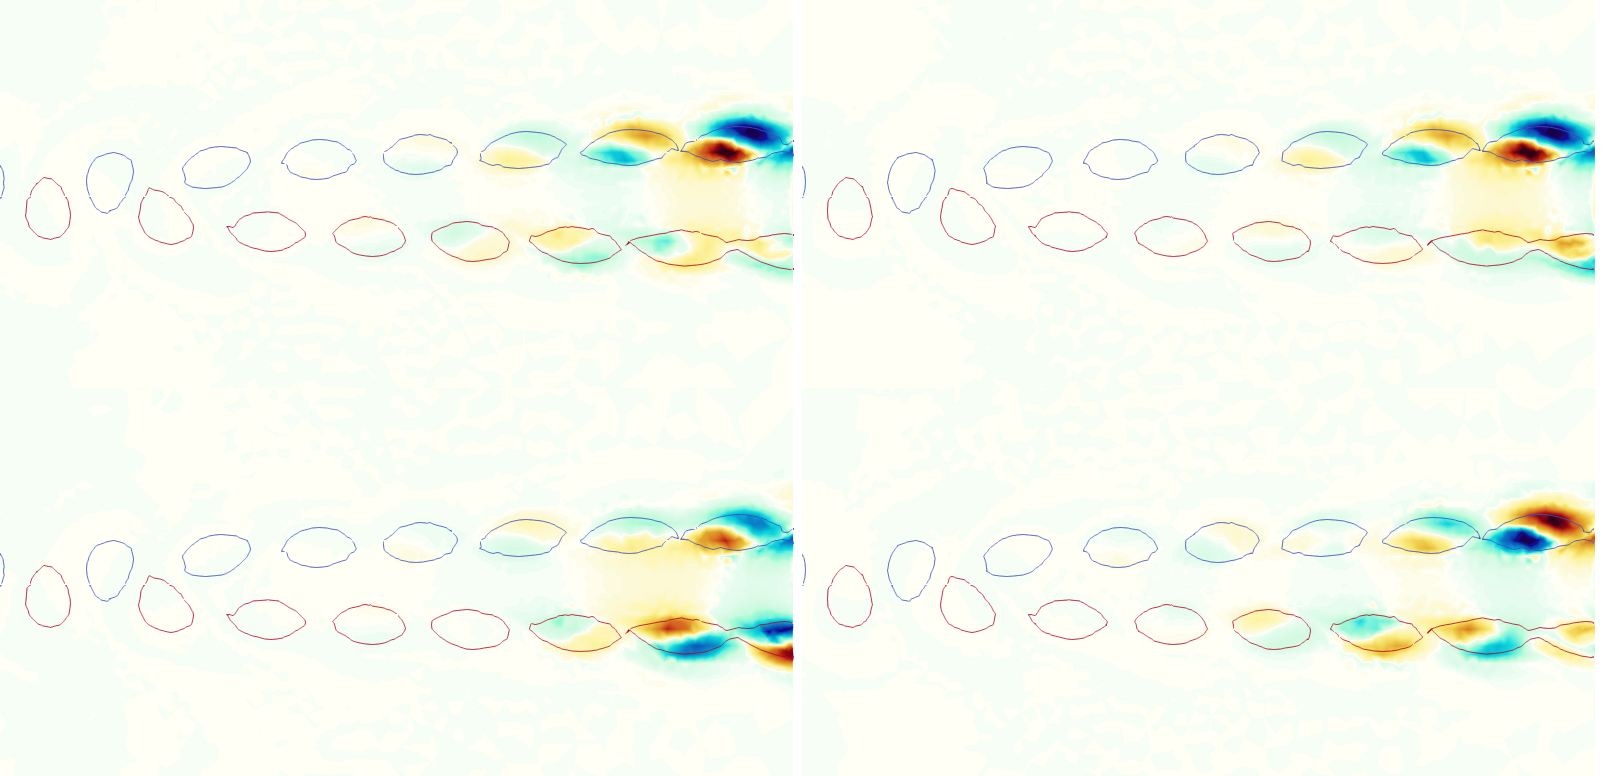
\includegraphics[width=1.0\textwidth]{./fig/AR3/Floquet_modes_beta_0_Re495.png}
  \caption{Floquet analysis for $\AR=3$ and $Re=495$. Top: Floquet multilpiers for $\beta = 0$. Bottom: Modes associated with the $4$ multipliers outside the unit circumference.}
  \label{fig:AR3_Stab}
\end{figure}

\begin{itemize}
  \item For $\AR=3$ we observe that the wake becomes unstable in the far wake.
  \item Study Batchelor and Lamb. Look for instability of trains of vortices
  \item How can the far wake be influenced by the body? Porbaby we have this phenopmena also at different AR, and with different bodies, but it happens at conditions different from the one we observed, since the wake is already 3d, or, for example at AR=4, the wake become storta so we do not see this phenomenom.
\end{itemize}

\fi
